%_____________________________________________________________________________
%=============================================================================
% main.tex v9 (30-11-2015) \ldots dibuat oleh Lionov - Informatika FTIS UNPAR
% 
% Ini adalah file utama (main.tex), berisi perintah-perintah yang khusus 
% dibuat untuk template ini
%
% 			JANGAN MENGUBAH APAPUN DI DALAM FILE INI,
%			KECUALI ANDA TAHU APA YANG ANDA LAKUKAN !!!
%
% Perubahan pada versi 9 (30-11-2015):
%	- bagian untuk menambahkan perintah sendiri dipindahkan ke data.tex
%	- bagian untuk mengatur kemunculan daftar gambar dan daftar tabel, dipindahkan
%	  ke data.tex
%	- penambahan bagian untuk mengatur perbedaan pdfTeX, masalah hfill dgn hfil
%	- bagian pengesahan diatur agar lebih rapi 
%
% Perubahan pada versi sebelumnya dapat dilihat di bagian akhir file ini
%_____________________________________________________________________________
%=============================================================================

%setup.tex
\documentclass[11pt,a4paper,twoside,openright,notitlepage]{report} 

\usepackage[bahasa]{babel} %bahasa indonesia
\usepackage[T1]{fontenc}  %encoding
% \usepackage{mathptmx}
% \usepackage{venturisold}
% \usepackage{helvet}
% \usepackage{fouriernc} 
\usepackage{abstract} %manipulasi abstract
\usepackage{chappg} % format daftar isi 
\usepackage{color} %warna
\usepackage{etoolbox} %untuk programming if-then
\usepackage{fancyhdr} %format header & footer
\usepackage{float} %penempatan gambar di tempat yg seharusnya
\usepackage[inner=2.5cm,outer=2cm,top=2.5cm,bottom=2.5cm]{geometry} %margin
\usepackage{graphicx} %gambar
\usepackage{listings} %source code
\usepackage{lscape} %landscape untuk source code
\usepackage{multicol} %multiple column
\usepackage{ifthen} % if then
\usepackage[pagewise]{lineno} %line numbering
\usepackage{lipsum} % untuk testing
\usepackage{titlesec} %judul header
\usepackage{tocbibind} %daftar isi, gambar, tabel dll
\usepackage{tocloft} % format daftar isi 
\usepackage{setspace} %line spacing
\usepackage{xstring} %manipulasi string
\usepackage[plainpages=false,pdfpagelabels,unicode]{hyperref} %\autoref, \phantomsection & link 
\usepackage{emptypage} %halaman kosong antar bab

\let\abstractname\Abstrak

\titleformat{\chapter}[display] {\Large\bfseries\centering}{\MakeUppercase{\chaptertitlename} \thechapter}{15pt}{\Large\MakeUppercase}

\renewcommand{\cftchapfont}{\scshape \bfseries}

\newcommand{\vdierror}{}
\newcommand{\daftarIsiError}[1]{\renewcommand{\vdierror}{#1}}

\ifdefempty{\vdierror}
	{\renewcommand{\cfttoctitlefont}{\hfil\Large\bfseries\MakeUppercase}}
	{\renewcommand{\cfttoctitlefont}{\hfil\Large\bfseries\MakeUppercase}}
\renewcommand{\cftaftertoctitle}{\hfill}
\renewcommand{\cftloftitlefont}{\hfill\Large\bfseries\MakeUppercase}
\renewcommand{\cftafterloftitle}{\hfill}
\renewcommand{\cftlottitlefont}{\hfill\Large\bfseries\MakeUppercase}
\renewcommand{\cftafterlottitle}{\hfill}

% Tidak perlu ada kata "Bab", "Gambar" atau "Tabel" di daftar 
% \renewcommand{\cftchappresnum}{{\bf \scshape Bab} } 
% \renewcommand{\cftchapnumwidth}{1.5cm}
% \renewcommand{\cftfigpresnum}{{Gambar\ }} 
% \renewcommand{\cftfignumwidth}{2.5cm}
% \renewcommand{\cfttabpresnum}{{Tabel\ }} 
% \renewcommand{\cfttabnumwidth}{2cm}

\newcommand{\apptoc}{
	% Hapus kata "Lampiran" dari daftar isi
	%\addtocontents{toc}{\protect\renewcommand{\protect\cftchappresnum}{\bf \scshape Lampiran\  }}%
	%\addtocontents{toc}{\protect\renewcommand{\protect\cftchapnumwidth}{2.75cm}}
	\addtocontents{toc}{\protect\renewcommand{\protect\cftchappresnum}{\bf \scshape}}%	
}

\newcommand{\vnama}{Jane Doe}
\newcommand{\vlnama}{John Doe}
\newcommand{\vnpm}{1992700001}
\newcommand{\vprodiINA}{SAINS}
\newcommand{\vprodiENG}{SCIENCE}
\newcommand{\vstaINA}{UJIAN}
\newcommand{\vstaENG}{EXAM}
%\newcommand{\vjudul}{Judul Skripsi/Tugas Akhir}
\newcommand{\vpembu}{Plato}
\newcommand{\vpembs}{Euclid}
\newcommand{\vpengi}{Plato}
\newcommand{\vpengii}{Euclid}
\newcommand{\vtanggal}{1}
\newcommand{\vbulan}{Januari}
\newcommand{\vtahun}{1970}
\newcommand{\vmode}{final}
\newcommand{\vspacing}{double}
\newcommand{\vlineno}{yes}
\newcommand{\vkunciina}{Skripsi, Tugas Akhir}
\newcommand{\vkuncieng}{Undergraduate Thesis, Final Project}
\newcommand{\vkajur}{Jack Doe}
\newcommand{\vkajurmat}{Jack Doe}
\newcommand{\vkajurfis}{Jack Doe}
\newcommand{\vkajurtif}{Jack Doe}
\newcommand{\vtabel}{}
\newcommand{\vgambar}{}

\newcommand{\namanpm}[2]{
	\renewcommand{\vstaINA}{<<SKRIPSI/TUGAS AKHIR>>}
	\renewcommand{\vprodiINA}{<<MATEMATIKA/FISIKA/TEKNIK INFORMATIKA>>}
	\renewcommand{\vstaENG}{<<FINAL PROJECT/UNDERGRADUATE THESIS>>}
	\renewcommand{\vprodiENG}{<<MATHEMATICS/PHYSICS/INFORMATICS>>}
	\renewcommand{\vnama}{\uppercase{#1}} \renewcommand{\vlnama}{#1} \hypersetup{pdfauthor={#2 - #1}}
	\renewcommand{\vnpm}{#2} \hypersetup{pdfcreator={#2}} \StrChar{\vnpm}{6}[\vprodiN]
	\ifdefstring{\vprodiN}{1}{
		\renewcommand{\vprodiINA}{MATEMATIKA} \renewcommand{\vprodiENG}{MATHEMATICS} 
		\renewcommand{\vstaINA}{SKRIPSI} \renewcommand{\vstaENG}{FINAL PROJECT} \renewcommand{\vkajur}{\vkajurmat}}{}
	\ifdefstring{\vprodiN}{2}{
		\renewcommand{\vprodiINA}{FISIKA} \renewcommand{\vprodiENG}{PHYSICS} 
		\renewcommand{\vstaINA}{TUGAS AKHIR} \renewcommand{\vstaENG}{FINAL PROJECT} \renewcommand{\vkajur}{\vkajurfis}}{}
	\ifdefstring{\vprodiN}{3}{
		\renewcommand{\vprodiINA}{TEKNIK INFORMATIKA} \renewcommand{\vprodiENG}{INFORMATICS} 
		\renewcommand{\vstaINA}{SKRIPSI} \renewcommand{\vstaENG}{UNDERGRADUATE THESIS} \renewcommand{\vkajur}{\vkajurtif}}{}
	}

%\newcommand{\judul}[1]{\renewcommand{\vjudul}{\uppercase{#1}}\hypersetup{pdftitle={#1}, pdfsubject={#1}}}
\newcommand{\pembimbing}[2]{\renewcommand{\vpembu}{#1}\renewcommand{\vpembs}{#2}}
\newcommand{\penguji}[2]{\renewcommand{\vpengi}{#1}\renewcommand{\vpengii}{#2}}
\newcommand{\kajur}[3]{\renewcommand{\vkajurmat}{#1}\renewcommand{\vkajurfis}{#2}\renewcommand{\vkajurtif}{#3}}
\renewcommand{\vbulan}{<<bulan>>}
\newcommand{\tanggal}[3]{\renewcommand{\vtanggal}{#1}\renewcommand{\vtahun}{#3}
	\newcommand{\vcbulan}{#2}
	\ifdefstring{\vcbulan}{1}{\renewcommand{\vbulan}{Januari}}{}
	\ifdefstring{\vcbulan}{2}{\renewcommand{\vbulan}{Februari}}{}
	\ifdefstring{\vcbulan}{3}{\renewcommand{\vbulan}{Maret}}{}
	\ifdefstring{\vcbulan}{4}{\renewcommand{\vbulan}{April}}{}
	\ifdefstring{\vcbulan}{5}{\renewcommand{\vbulan}{Mei}}{}
	\ifdefstring{\vcbulan}{6}{\renewcommand{\vbulan}{Juni}}{}
	\ifdefstring{\vcbulan}{7}{\renewcommand{\vbulan}{Juli}}{}
	\ifdefstring{\vcbulan}{8}{\renewcommand{\vbulan}{Agustus}}{}
	\ifdefstring{\vcbulan}{9}{\renewcommand{\vbulan}{September}}{}
	\ifdefstring{\vcbulan}{10}{\renewcommand{\vbulan}{Oktober}}{}
	\ifdefstring{\vcbulan}{11}{\renewcommand{\vbulan}{November}}{}
	\ifdefstring{\vcbulan}{12}{\renewcommand{\vbulan}{Desember}}{}	
}

\newcommand{\judulINA}[1]{\newcommand{\vjudulINA}{\uppercase{#1}}\hypersetup{pdftitle={#1},pdfsubject={#1}}}
\newcommand{\judulENG}[1]{\newcommand{\vjudulENG}{\uppercase{#1}}\hypersetup{pdftitle={#1},pdfsubject={#1}}}
\newcommand{\abstrakINA}[1]{\newcommand{\vabstrakina}{#1}}
\newcommand{\abstrakENG}[1]{\newcommand{\vabstrakeng}{#1}}
\newcommand{\kunciINA}[1]{\renewcommand{\vkunciina}{#1} \hypersetup{pdfkeywords={#1}}}
\newcommand{\kunciENG}[1]{\renewcommand{\vkuncieng}{#1}}
\newcommand{\untuk}[1]{\newcommand{\vuntuk}{#1}}
\newcommand{\prakata}[1]{\newcommand{\vprakata}{#1}}
\newcommand{\mode}[1]{\renewcommand{\vmode}{#1}}
\newcommand{\linespacing}[1]{\renewcommand{\vspacing}{#1}}
\newcommand{\linenumber}[1]{\renewcommand{\vlineno}{#1}}

\newcommand{\gambar}[1]{\renewcommand{\vgambar}{#1}}
\newcommand{\tabel}[1]{\renewcommand{\vtabel}{#1}}

\newcommand{\bab}[1]{\newcommand{\vbab}{#1}}
\newcommand{\lampiran}[1]{\renewcommand{\vlmp}{#1}}

\newcommand{\vpilbab}{0}
\newcommand{\vbaba}{0}\newcommand{\vbabb}{0}\newcommand{\vbabc}{0}
\newcommand{\vbabd}{0}\newcommand{\vbabe}{0}\newcommand{\vbabf}{0}
\newcommand{\vbabg}{0}\newcommand{\vbabh}{0}\newcommand{\vbabi}{0}
\newcommand{\vpillmp}{0}
\newcommand{\vlmpa}{0}\newcommand{\vlmpb}{0}\newcommand{\vlmpc}{0}
\newcommand{\vlmpd}{0}\newcommand{\vlmpe}{0}\newcommand{\vlmpf}{0}
\newcommand{\vlmpg}{0}\newcommand{\vlmph}{0}\newcommand{\vlmpi}{0}
\newcommand{\vlmp}{x}

%	\ifdefempty{#1}{\bab{1,2,3,4,5,6,7,8,9} \tampilbab{\vbab}}{
\newcommand{\tampilbab}[1]{
	\ifdefempty{#1}{
		\renewcommand{\vbaba}{1}\renewcommand{\vbabb}{1}\renewcommand{\vbabc}{1}
		\renewcommand{\vbabd}{1}\renewcommand{\vbabe}{1}\renewcommand{\vbabf}{1}
		\renewcommand{\vbabg}{1}\renewcommand{\vbabh}{1}\renewcommand{\vbabi}{1}}{
	\renewcommand{\do}[1]{
		\renewcommand{\vpilbab}{##1}
		\ifdefstring{\vpilbab}{1}{\renewcommand{\vbaba}{1}}{}
		\ifdefstring{\vpilbab}{2}{\renewcommand{\vbabb}{1}}{}
		\ifdefstring{\vpilbab}{3}{\renewcommand{\vbabc}{1}}{}
		\ifdefstring{\vpilbab}{4}{\renewcommand{\vbabd}{1}}{}
		\ifdefstring{\vpilbab}{5}{\renewcommand{\vbabe}{1}}{}
		\ifdefstring{\vpilbab}{6}{\renewcommand{\vbabf}{1}}{}
		\ifdefstring{\vpilbab}{7}{\renewcommand{\vbabg}{1}}{}
		\ifdefstring{\vpilbab}{8}{\renewcommand{\vbabh}{1}}{}
		\ifdefstring{\vpilbab}{9}{\renewcommand{\vbabi}{1}}{}
	}
	\expandafter\docsvlist\expandafter{#1}
	}
}

\newcommand{\tampillmp}[1]{
	\ifdefempty{#1}{
		\renewcommand{\vlmpa}{1}\renewcommand{\vlmpb}{1}\renewcommand{\vlmpc}{1}
		\renewcommand{\vlmpd}{1}\renewcommand{\vlmpe}{1}\renewcommand{\vlmpf}{1}
		\renewcommand{\vlmpg}{1}\renewcommand{\vlmph}{1}\renewcommand{\vlmpi}{1}}{
	\ifdefstring{#1}{-1}{ }{
		\renewcommand{\do}[1]{ 
			\renewcommand{\vpillmp}{##1}
			\ifdefstring{\vpillmp}{A}{\renewcommand{\vlmpa}{1}}{}
			\ifdefstring{\vpillmp}{B}{\renewcommand{\vlmpb}{1}}{}
			\ifdefstring{\vpillmp}{C}{\renewcommand{\vlmpc}{1}}{}
			\ifdefstring{\vpillmp}{D}{\renewcommand{\vlmpd}{1}}{}
			\ifdefstring{\vpillmp}{E}{\renewcommand{\vlmpe}{1}}{}
			\ifdefstring{\vpillmp}{F}{\renewcommand{\vlmpf}{1}}{}
			\ifdefstring{\vpillmp}{G}{\renewcommand{\vlmpg}{1}}{}
			\ifdefstring{\vpillmp}{H}{\renewcommand{\vlmph}{1}}{}
			\ifdefstring{\vpillmp}{I}{\renewcommand{\vlmpi}{1}}{}}
		}
	\expandafter\docsvlist\expandafter{#1}
	}
}

\newcommand{\appspacing}{
	\ifdefstring{\vspacing}{single}{\singlespacing}{}
	\ifdefstring{\vspacing}{onehalf}{\onehalfspacing}{}
	\ifdefstring{\vspacing}{double}{\doublespacing}{}
	\ifdefstring{\vmode}{final}{\onehalfspacing}{}
}

\newcommand{\appline}{
	\ifdefstring{\vmode}{final}{\renewcommand{\vlineno}{no}}{}
	\ifdefstring{\vlineno}{yes}{\linenumbers \def\linenumberfont{\normalfont\tiny\sffamily}}{}
	\ifdefstring{\vlineno}{no}{\lstset{numbers=left, stepnumber=1, numbersep=5pt}}{}
	
}

\newcommand{\appmargin}{
	\ifdefstring{\vmode}{final}{}{\newgeometry{inner=3cm,outer=2.75cm,top=2cm,bottom=2cm}}
}

\renewcommand{\abstractnamefont}{\bf \MakeUppercase}

\makeatletter
\def\headrule{{%
  \if@fancyplain\let\headrulewidth\plainheadrulewidth\fi
  \hrule\@height\footrulewidth\@width\headwidth\vskip2pt%
  \hrule\@height\headrulewidth\@width\headwidth\vskip-\headrulewidth\vskip-4pt
}}
\def\footrule{}

\def\cleardoublepage{
	\clearpage
	\if@twoside \ifodd\c@page
	\else
		\hbox{}
		\vspace{\fill} 
		\thispagestyle{empty}
		\newpage
	\if@twocolumn\hbox{}\newpage\fi\fi\fi}
\makeatother

\renewcommand{\headrulewidth}{1.25pt}
\renewcommand{\footrulewidth}{0.25pt}

\setlength{\headheight}{15pt}
\fancyhead[LE,RO]{\thepage}
\fancyhead[RE]{\small{\textsc{\nouppercase{\leftmark}}}}
\fancyhead[LO]{\small{\textsc{\nouppercase{\rightmark}}}}
\fancyfoot{}

\hypersetup{unicode=true,colorlinks=true,linkcolor=blue,citecolor=green,filecolor=magenta, urlcolor=cyan}

\lstset{basicstyle=\tiny, commentstyle=\color{blue}}
\lstset{frame=leftline, tabsize=4, breaklines=true}

%end setup.tex

%_____________________________________________________________________________
%=============================================================================
% data.tex v7 (30-11-2015) \ldots dibuat oleh Lionov - Informatika FTIS UNPAR
%
% Perubahan pada versi 7 (30-11-2015)
%	- Perubahan nomor bagian karena penyisipan Bagian V
%	- Penambahan Bagian V : pengaturan kemunculan daftar gambar dan/atau tabel 
%	  dipindahkan dari main.tex
%	- Penambahan Bagian XV : tempat untuk menambahkan perintah yang dibuat 
%	  sendiri, dipindahkan dari main.tex
%	- Penambahan Bagian 0 : perintah bagi yang caption daftar isi tidak bisa
%	  ke bagian tengah
%
% Perubahan pada versi sebelumnya dapat dilihat di bagian akhir file ini
%_____________________________________________________________________________
%=============================================================================

%=============================================================================
% 								PETUNJUK
%=============================================================================
% Ini adalah file data (data.tex)
% Masukkan ke dalam file ini, data-data yang diperlukan oleh template ini
% Cara memasukkan data dijelaskan di setiap bagian
% Data yang WAJIB dan HARUS diisi dengan baik dan benar adalah SELURUHNYA !!
% Hilangkan tanda << dan >> jika anda menemukannya
%=============================================================================

%_____________________________________________________________________________
%=============================================================================
% 								BAGIAN 0
%=============================================================================
% PERHATIAN!! PERHATIAN!! Bagian ini hanya ada untuk sementara saja
% Jika "DAFTAR ISI" tidak bisa berada di bagian tengah halaman, isi dengan XXX
% jika sudah benar posisinya, biarkan kosong (i.e. \daftarIsiError{ })
%=============================================================================
\daftarIsiError{ }
%=============================================================================

%_____________________________________________________________________________
%=============================================================================
% 								BAGIAN I
%=============================================================================
% Tambahkan package2 lain yang anda butuhkan di sini
%=============================================================================
\usepackage{booktabs} 
\usepackage[table]{xcolor}
\usepackage{longtable}
\usepackage{amsmath}
\usepackage{todo}
%=============================================================================

%_____________________________________________________________________________
%=============================================================================
% 								BAGIAN II
%=============================================================================
% Mode dokumen: menetukan halaman depan dari dokumen, apakah harus mengandung 
% prakata/pernyataan/abstrak dll (termasuk daftar gambar/tabel/isi) ?
% - kosong : tidak ada halaman depan sama sekali (untuk dokumen yang 
%            dipergunakan pada proses bimbingan)
% - cover : cover saja tanpa daftar isi, gambar dan tabel
% - sidang : cover, daftar isi, gambar, tabel (IT: UTS-UAS Seminar 
%			 dan UTS TA)
% - sidang_akhir : mode sidang + abstrak + abstract
% - final : seluruh halaman awal dokumen (untuk cetak final)
% Jika tidak ingin mencetak daftar tabel/gambar (misalkan karena tidak ada 
% isinya), edit manual di baris 439 dan 440 pada file main.tex
%=============================================================================
% \mode{kosong}
% \mode{cover}
% \mode{sidang}
%\mode{sidang_akhir}
\mode{final} 
%=============================================================================

%_____________________________________________________________________________
%=============================================================================
% 								BAGIAN III
%=============================================================================
% Line numbering: penomoran setiap baris, otomatis di-reset setiap berganti
% halaman
% - yes: setiap baris diberi nomor
% - no : baris tidak diberi nomor, otomatis untuk mode final
%=============================================================================
\linenumber{yes}
%=============================================================================

%_____________________________________________________________________________
%=============================================================================
% 								BAGIAN IV
%=============================================================================
% Linespacing: jarak antara baris 
% - single: opsi yang disediakan untuk bimbingan, jika pembimbing tidak
%            keberatan (untuk menghemat kertas)
% - onehalf: default dan wajib (dan otomatis) jika ingin mencetak dokumen
%            final/untuk sidang.
% - double : jarak yang lebih lebar lagi, jika pembimbing berniat memberi 
%            catatan yg banyak di antara baris (dianjurkan untuk bimbingan)
%=============================================================================
\linespacing{single}
%\linespacing{onehalf}
%\linespacing{double}
%=============================================================================

%_____________________________________________________________________________
%=============================================================================
% 								BAGIAN V
%=============================================================================
% Tidak semua skripsi memuat gambar dan/atau tabel. Untuk skripsi yang seperti
% itu, tidak diperlukan Daftar Gambar dan Daftar Tabel. Sayangnya hal ini 
% sulit dilakukan secara manual karena membutuhkan kedisiplinan pengguna 
% template.  
% Jika tidak akan menampilkan Daftar Gambar/Tabel, isi dengan NO. Jika ingin
% menampilkan, kosongkan parameter (i.e. \gambar{ }, \tabel{ })
%=============================================================================
\gambar{ }
\tabel{ }
%=============================================================================

%_____________________________________________________________________________
%=============================================================================
% 								BAGIAN VI
%=============================================================================
% Bab yang akan dicetak: isi dengan angka 1,2,3 s.d 9, sehingga bisa digunakan
% untuk mencetak hanya 1 atau beberapa bab saja
% Jika lebih dari 1 bab, pisahkan dengan ',', bab akan dicetak terurut sesuai 
% urutan bab (e.g. \bab{1,2,3}).
% Untuk mencetak seluruh bab, kosongkan parameter (i.e. \bab{ })  
% Catatan: Jika ingin menambahkan bab ke-10 dan seterusnya, harus dilakukan 
% secara manual
%=============================================================================
\bab{ }
%=============================================================================

%_____________________________________________________________________________
%=============================================================================
% 								BAGIAN VII
%=============================================================================
% Lampiran yang akan dicetak: isi dengan huruf A,B,C s.d I, sehingga bisa 
% digunakan untuk mencetak hanya 1 atau beberapa lampiran saja
% Jika lebih dari 1 lampiran, pisahkan dengan ',', lampiran akan dicetak 
% terurut sesuai urutan lampiran (e.g. \bab{A,B,C}).
% Jika tidak ingin mencetak lampiran apapun, isi dengan -1 (i.e. \lampiran{-1})
% Untuk mencetak seluruh mapiran, kosongkan parameter (i.e. \lampiran{ })  
% Catatan: Jika ingin menambahkan lampiran ke-J dan seterusnya, harus 
% dilakukan secara manual
%=============================================================================
\lampiran{ }
%=============================================================================

%_____________________________________________________________________________
%=============================================================================
% 								BAGIAN VIII
%=============================================================================
% Data diri dan skripsi/tugas akhir
% - namanpm: Nama dan NPM anda, penggunaan huruf besar untuk nama harus benar
%			 dan gunakan 10 digit npm UNPAR, PASTIKAN BAHWA BENAR !!!
%			 (e.g. \namanpm{Jane Doe}{1992710001}
% - judul : Dalam bahasa Indonesia, perhatikan penggunaan huruf besar, judul
%			tidak menggunakan huruf besar seluruhnya !!! 
% - tanggal : isi dengan {tangga}{bulan}{tahun} dalam angka numerik, jangan 
%			  menuliskan kata (e.g. AGUSTUS) dalam isian bulan
%			  Tanggal ini adalah tanggal dimana anda akan melaksanakan sidang 
%			  ujian akhir skripsi/tugas akhir
% - pembimbing: isi dengan pembimbing anda, lihat daftar dosen di file dosen.tex
%				jika pembimbing hanya 1, kosongkan parameter kedua 
%				(e.g. \pembimbing{\JND}{  } ) , \JND adalah kode dosen
% - penguji : isi dengan para penguji anda, lihat daftar dosen di file dosen.tex
%				(e.g. \penguji{\JHD}{\JCD} ) , \JND dan \JCD adalah kode dosen
% !!Lihat singkatan pembimbing dan penguji anda di file dosen.tex
%=============================================================================
\namanpm{Yohanes Mario Chandra}{2011730031}	%hilangkan tanda << & >>
\tanggal{1}{8}{2016}			%hilangkan tanda << & >>
\pembimbing{\PAS}{} %hilangkan tanda << & >>    
\penguji{<<penguji 1>>}{<<penguji 2>>} 				%hilangkan tanda << & >>
%=============================================================================

%_____________________________________________________________________________
%=============================================================================
% 								BAGIAN IX
%=============================================================================
% Judul dan title : judul bhs indonesia dan inggris
% - judulINA: judul dalam bahasa indonesia
% - judulENG: title in english
% PERHATIAN: - langsung mulai setelah '{' awal, jangan mulai menulis di baris 
%			   bawahnya
%			 - Gunakan \texorpdfstring{\\}{} untuk pindah ke baris baru
%			 - Judul TIDAK ditulis dengan menggunakan huruf besar seluruhnya !!
%			 - Gunakan perintah \texorpdfstring{\\}{} untuk baris baru
%=============================================================================
\judulINA{Perangkat Lunak Login Otomatis \texorpdfstring{\\}{} Untuk \textit{Captive Portal} Wi-Fi}
\judulENG{Automated Login Software \texorpdfstring{\\}{} For Wi-Fi Captive Portal}
%_____________________________________________________________________________
%=============================================================================
% 								BAGIAN X
%=============================================================================
% Abstrak dan abstract : abstrak bhs indonesia dan inggris
% - abstrakINA: abstrak bahasa indonesia
% - abstrakENG: abstract in english
% PERHATIAN: langsung mulai setelah '{' awal, jangan mulai menulis di baris 
%			 bawahnya
%=============================================================================
\abstrakINA{<<Tuliskan abstrak anda di sini, dalam bahasa Indonesia>> \lipsum[5]}
\abstrakENG{<<Tuliskan abstrak anda di sini, dalam bahasa Inggris>> \lipsum[5]} 
%=============================================================================

%_____________________________________________________________________________
%=============================================================================
% 								BAGIAN XI
%=============================================================================
% Kata-kata kunci dan keywords : diletakkan di bawah abstrak (ina dan eng)
% - kunciINA: kata-kata kunci dalam bahasa indonesia
% - kunciENG: keywords in english
%=============================================================================
\kunciINA{<<Tuliskan di sini kata-kata kunci yang anda gunakan, dalam bahasa Indonesia>>}
\kunciENG{<<Tuliskan di sini kata-kata kunci yang anda gunakan, dalam bahasa Inggris>>}
%=============================================================================

%_____________________________________________________________________________
%=============================================================================
% 								BAGIAN XII
%=============================================================================
% Persembahan : kepada siapa anda mempersembahkan skripsi ini ...
%=============================================================================
\untuk{<<kepada siapa anda mempersembahkan skripsi ini\ldots?>>}
%=============================================================================

%_____________________________________________________________________________
%=============================================================================
% 								BAGIAN XIII
%=============================================================================
% Kata Pengantar: tempat anda menuliskan kata pengantar dan ucapan terima 
% kasih kepada yang telah membantu anda bla bla bla ....  
%=============================================================================
\prakata{\lipsum[3]}
%=============================================================================

%_____________________________________________________________________________
%=============================================================================
% 								BAGIAN XIV
%=============================================================================
% Tambahkan hyphen (pemenggalan kata) yang anda butuhkan di sini 
%=============================================================================
\hyphenation{ma-te-ma-ti-ka}
\hyphenation{fi-si-ka}
\hyphenation{tek-nik}
\hyphenation{in-for-ma-ti-ka}
\hyphenation{web-brow-ser}
\hyphenation{pass-word-vault}
%=============================================================================

%_____________________________________________________________________________
%=============================================================================
% 								BAGIAN XV
%=============================================================================
% Tambahkan perintah yang anda buat sendiri di sini 
%=============================================================================
\newcommand{\vtemplateauthor}{lionov}
%=============================================================================

%=============================================================================
% Perubahan pada versi 6 (13-04-2015)
% 	- Perubahan untuk data-data ``template" menjadi lebih generik dan 
%	  menggunakan tanda << dan >>
% Perubahan pada versi 5 (10-11-2013)
% 	- Perbaikan pada memasukkan bab : tidak perlu menuliskan apapun untuk 
%	  memasukkan seluruh bab (bagian V)
% 	- Perbaikan pada memasukkan lampiran : tidak perlu menuliskan apapun untuk
%	  memasukkan seluruh lampiran atau -1 jika tidak memasukkan apapun
% Perubahan pada versi 4 (21-10-2012)
%	- Data dosen dipindah ke dosen.tex agar jika ada perubahan/update data 
%	  dosen, mahasiswa tidak perlu mengubah data.tex
%	- Perubahan pada keterangan dosen	
% Perubahan pada versi 3 (06-08-2012)
% 	- Perubahan pada beberapa keterangan 
% Perubahan pada versi 2 (09-07-2012):
% 	- Menambahkan data judul dalam bahasa inggris
% 	- Membuat bagian khusus untuk judul (bagian VIII)
% 	- Perbaikan pada gelar dosen
% Versi 1 (08-11-2011)
%=============================================================================
%_____________________________________________________________________________
%=============================================================================
% dosen.tex v5 (30-11-2015) \ldots dibuat oleh Lionov - Informatika FTIS UNPAR
%
% Perubahan pada versi 5 (30-11-2015)
% 	- Perubahan ketua jurusan matematika menjadi JDL
% 	- Perubahan ketua jurusan teknik informatika menjadi MAR
%	- Penghapusan dosen (Hariman,Farica,Lukcy,Verli,Wahyu)
%	- Penambahan dosen (Risti, Bagoes, Reinard, Haryanto)
%	- Perbaikan gelar (Ferry, Rusli, Fla, Kian Ming, Wono, Gede, Pascal)
%	- Penggunaan thin-space untuk spasi pada nama, agar tidak terpotong
%
% Perubahan pada versi sebelumnya dapat dilihat di bagian akhir file ini
%_____________________________________________________________________________
%=============================================================================

%=============================================================================
% Data dosen dan kajur FTIS - JANGAN MENGUBAH APAPUN DI BAGIAN INI, KECUALI
% untuk mengubah kajur (jika kajur telah berganti orang) atau menambahkan 
% pembimbing anda yang tidak/belum tercantum pada daftar ini atau 
% memperbaiki penulisan gelar jika penguji anda meminta
% perintah: \kajur{1}{2}{3} 1: Matematika 2: Fisika 3: Teknik Informatika
%=============================================================================
% CATATAN UNTUK MAHASISWA TEKNIK INFORMATIKA :
% dosen yang ditandai * :
% - jika menjadi penguji,tetap,hapus komentar (tanda % dan *) agar dapat digunakan
% - jika menjadi pembimbing, harus diganti namanya dengan dosen lain, ikuti
% 	petunjuk dari koordinator Skripsi !
% - khusus untuk MAR, harus diganti juga sesuai petunjuk koordinator
%=============================================================================

\kajur{\JDL}{\PNG}{Mariskha\,Tri\,Adithia,\,P.D.Eng} 

%dummy person
\newcommand{\JND}{Jane\,Doe} 
\newcommand{\JHD}{John\,Doe}
\newcommand{\JCD}{Jack\,Doe}

% Dosen-dosen Program Studi Matematika
\newcommand{\JDL}{Dr.\,Julius\,Dharma\,Lesmono}
\newcommand{\FAR}{Farah\,Kristiani,\,M.Si.}
\newcommand{\ERW}{Erwinna\,Chendra,\,M.Si.}
\newcommand{\FJP}{Dr.\,Ferry\,Jaya\,Permana,\,ASAI}
\newcommand{\AGS}{Agus\,Sukmana,\,M.Sc.}
\newcommand{\WSB}{Prof.\,M.\,Wono\,Setya\,Budhi,\,Ph.D.}
\newcommand{\LIM}{Liem\,Chin,\,M.Si.}
\newcommand{\IWS}{Iwan\,Sugiarto,\,M.Si.}
\newcommand{\IVM}{Ivonne\,Martin,\,M.Sc.}
\newcommand{\OWN}{Livia\,Owen,\,M.Si.}
\newcommand{\BNY}{Benny\,Yong,\,M.Si.}
\newcommand{\TFK}{Taufik\,Limansyah,\,M.T.}
\newcommand{\MRA}{Maria\,Anestasia,\,M.Si.}

% Dosen-dosen Program Studi Fisika
\newcommand{\PCT}{Paulus\,Cahyono\,Tjiang,\,Ph.D.}
\newcommand{\BSB}{Prof.\,B.\,Suprapto\,Brotosiswojo,\,Ph.D.}
\newcommand{\RUS}{Aloysius\,Rusli,\,Ph.D.}
\newcommand{\KMG}{Kian\,Ming,\,M.Si.}
\newcommand{\SHS}{Sylvia\,Hastuti\,Sutanto,\,Ph.D.}
\newcommand{\JVS}{Janto\,Vincent\,Sulungbudi,\,S.Si.}
\newcommand{\FLA}{Flaviana,\,M.T.}
\newcommand{\PNG}{Philips\,Nicolas\,Gunawidjaja,\,Ph.D.}
\newcommand{\ELK}{Elok\,Fidiani,\,M.Sc.}
\newcommand{\RIS}{Risti\,Suryantari,\,M.Sc.}
\newcommand{\HAS}{Haryanto\,Siahaan,\,Ph.D.}
\newcommand{\RND}{Reinard\,Primulando,\,Ph.D.}

% Dosen-dosen Program Studi Teknik Informatika
\newcommand{\CEN}{Dr.rer.nat.\,Cecilia\,Esti\,Nugraheni}
\newcommand{\VSM}{Dr.\,Veronica\,Sri\,Moertini}
\newcommand{\RDL}{Rosa\,De\,Lima,\,M.Kom.}
\newcommand{\TAB}{Dott.\,Thomas\,Anung\,Basuki}
\newcommand{\LNV}{Lionov,\,M.Sc.}
% \newcommand{\OSS}{Dr.\,Oerip\,S.\,Santoso}
% * \newcommand{\MAR}{Mariskha\,Tri\,Adithia,\,P.D.Eng}
\newcommand{\LCA}{Luciana\,Abednego,\,M.T.}
\newcommand{\ELH}{Elisati\,Hulu,\,M.T.}
% * \newcommand{\CAN}{Chandra\,Wijaya,\,M.T.}
\newcommand{\GDK}{Gede\,Karya,\,M.T.,\,CISA}
\newcommand{\NIS}{Nico\,Saputro,\,M.T.}
% * \newcommand{\JNH}{Joanna\,Helga,\,M.Sc.}
\newcommand{\PAS}{Pascal\,Alfadian,\,M.Comp.} 
% * \newcommand{\HUS}{Husnul\,Hakim,\,M.T.} 
% * \newcommand{\VAN}{Vania\,Natali,\,M.T.} 
% * \newcommand{\BHR}{Aditya\,Bagoes\,Saputra,\,M.T.} 

%=============================================================================
% Perubahan pada versi 4 (01-03-2014)
% 	- Perubahan ketua jurusan teknik informatika menjadi TAB
%	- Penambahan dosen jurusan informatika (Lucky)
%
% Perubahan pada versi 3 (10-11-2013)
% 	- Perubahan ketua jurusan teknik informatika menjadi MAR
%	- Penambahan dosen jurusan informatika (Joanna, Wahyu)
%	- Penghapusan dosen informatika (Lucky, Dharu)
%
% Perubahan pada versi 2 (25-02-2013)
% 	- Tambahan catatan untuk mhs T. Inf. terkait dosen yg tidak bisa menjadi pemb.
% 	- Update data gelar untuk Taufik (MAT)
% 	- Penambahan baru (Farica-Fisika, Husnul-T.Informatika)
% 	- Dosen keluar atau tidak menjadi pembimbing lagi (Nisa, Ghifary)
%
% Versi 1 (21-10-2012)
% 	- Data dosen dipindah dari data.tex agar jika ada perubahan/update data dosen
%     mahasiswa tidak perlu mengubah data.tex
% 	- Beberapa dosen Informatika yang tidak boleh menjadi pembimbing digantikan OSS
% 	- Update data gelar untuk Maria (MAT)
% 	- Penambahan baru (Flaviana-Fisika, Elok-Fisika)
% 	- Dosen keluar atau tidak menjadi pembimbing lagi (Monika, David)
%=============================================================================

\begin{document}

\raggedbottom

\def\bibname{Daftar Referensi}
\def\abstractname{Abstrak}

\pagestyle{empty}

%depan.tex
\ifdefstring{\vmode}{kosong}{}{

\pagenumbering{roman}

%cover INA
\begin{center}
	{\Large\bf \vstaINA \\} 	\vspace{1.5cm}
	{\Large \bf \vjudulINA \\} \vspace{2.5cm}
	\includegraphics[scale=0.4]{Gambar/logo-unpar}\\ \vspace{1cm}
	{\Large \bf \vnama \\} \vspace{0.5cm}
	{\Large \bf NPM: \vnpm \\}
	\vfill
	\Large{ \textbf { 
		PROGRAM STUDI \vprodiINA \\
		FAKULTAS TEKNOLOGI INFORMASI DAN SAINS\\
		UNIVERSITAS KATOLIK PARAHYANGAN\\
		\vtahun 
	}}
\end{center}
\cleardoublepage

%cover ENG
\begin{center}
	{\Large\bf \vstaENG \\} 	\vspace{1.5cm}
	{\Large \bf \vjudulENG \\} \vspace{2.5cm}
	\includegraphics[scale=0.4]{Gambar/logo-unpar}\\ \vspace{1cm}
	{\Large \bf \vnama \\} \vspace{0.5cm}
	{\Large \bf NPM: \vnpm \\}
	\vfill
	\Large{ \textbf { 
		DEPARTMENT OF \vprodiENG \\
		FACULTY OF INFORMATION TECHNOLOGY AND SCIENCES\\
		PARAHYANGAN CATHOLIC UNIVERSITY\\
		\vtahun 
	}}
\end{center}
\cleardoublepage


% Lembar pengesahan
\ifdefstring{\vmode}{final}{
\begin{center}
	{\Large\bf LEMBAR PENGESAHAN \\} 	\vspace{1.5cm}
	{\Large \bf \vjudulINA \\} 			\vspace{1cm}
	{\Large \bf \vnama \\}				\vspace{0.5cm}
	{\Large \bf NPM: \vnpm \\}			\vspace{1.5cm}
	\large{ \bfseries{
		\begin{centering} 
			Bandung, \vtanggal\ \vbulan\ \vtahun \\ \vspace{0.25cm} Menyetujui,\\
			\vspace{0.75cm}
			\ifdefempty{\vpembs}
					{\centering Pembimbing Tunggal\\ \vspace{2.25cm} \vpembu\\}
					{ 	\begin{minipage}[b]{0.46\linewidth}
							\centering Pembimbing Utama \\ \vspace{2.5cm} \vpembu \\
						\end{minipage} \hspace{0.5cm}
						\begin{minipage}[b]{0.46\linewidth}
							\centering Pembimbing Pendamping \\	\vspace{2.5cm} \vpembs \\
						\end{minipage}	
					}
		\end{centering}
		\vspace{1.5cm}
		\begin{centering}	
			\begin{minipage}[b]{0.46\linewidth}
				\centering Ketua Tim Penguji \\ \vspace{2.5cm} \vpengi \\
			\end{minipage} \hspace{0.5cm}
			\begin{minipage}[b]{0.46\linewidth}
				\centering Anggota Tim Penguji \\ \vspace{2.5cm} \vpengii 
			\end{minipage}
		\end{centering}
		\vspace{1.5cm} \\
		\centering Mengetahui,\\ \vspace{0.5cm}	
		Ketua Program Studi \\ \vspace{2.5cm} \vkajur\\
	}}			
\end{center}
\cleardoublepage

% Lembar Pernyataan
\vspace*{4cm}
{\Large\bf \centering PERNYATAAN\\} \vspace{1cm}
\noindent
Dengan ini saya yang bertandatangan di bawah ini menyatakan bahwa \MakeLowercase{\vstaINA} dengan judul:  \vspace{0.5cm}
\begin{center}
	{\large \bf \vjudulINA \\}
\end{center}
\vspace{0.75cm}
adalah benar-benar karya saya sendiri, dan saya tidak melakukan penjiplakan atau pengutipan dengan cara-cara yang tidak sesuai dengan etika keilmuan yang berlaku dalam masyarakat keilmuan.
			
Atas pernyataan ini, saya siap menanggung segala risiko dan sanksi yang dijatuhkan kepada saya, apabila di kemudian hari ditemukan adanya pelanggaran terhadap etika keilmuan dalam karya saya, atau jika ada tuntutan formal atau non-formal dari pihak lain berkaitan dengan keaslian karya saya ini.\\
\vspace{0.25cm}

\begin{flushright}	
	Dinyatakan di Bandung,\\
	Tanggal \vtanggal\ \vbulan\ \vtahun \\ \vspace{0.5cm}
	\begin{tabular}{|p{1.75cm}|}
		\hline
		\\ Meterai \\ \\  
		\hline
	\end{tabular}\\
	\vspace{0.5cm} 
	\vlnama \\
	NPM: \vnpm
\end{flushright}
 \cleardoublepage
}{}

% Abstrak & Abstract
\ifthenelse{{\equal{\vmode}{sidang_akhir}}\or{\equal{\vmode}{final}}}{
\ifdefempty{\vabstrakina}{}
	  { \vspace*{4cm}
		\begin{abstract}
			%\noindent \normalsize{\onehalfspacing{\vabstrakina \vspace*{1cm}\\
			\noindent \normalsize{\vabstrakina \vspace*{1cm} 
			
			{\noindent \bfseries Kata-kata kunci:\ } \vkunciina}
		\end{abstract}
  		\cleardoublepage
	  }
\ifdefempty{\vabstrakeng}{}
	  { \def\abstractname{Abstract}
		\vspace*{4cm}
		\begin{abstract}
			%\noindent \normalsize{\onehalfspacing{\vabstrakeng \vspace*{1cm}\\
			\noindent \normalsize{\vabstrakeng \vspace*{1cm} 
			
			{\noindent \bfseries Keywords:\ } \vkuncieng}
		\end{abstract}			
 		\cleardoublepage
	  }
}{}

% Lembar persembahan
\ifdefstring{\vmode}{final}{
\ifdefempty{\vuntuk}{}
	  { \vspace*{5cm}
		\begin{quote} 
			\em \raggedleft \Large{\vuntuk} 
		\end{quote}
 		\cleardoublepage
	  }

\pagestyle{plain}
	 
% Kata pengantar
\ifdefempty{\vprakata}{}
	  {	\chapter*{Kata Pengantar}
		\label{ch:prakata}
		\addcontentsline{toc}{chapter}{Kata Pengantar}
		\vprakata \vspace{0.25cm}
		\begin{flushright}	
			Bandung,\ \vbulan\ \vtahun \\ \vspace{1cm}
			Penulis \\
		\end{flushright}
		\cleardoublepage		
	  }
}{}

\ifthenelse{{\equal{\vmode}{kosong}}\or{\equal{\vmode}{cover}}}{}
	{ \tableofcontents \newpage 	% Daftar isi
	  \ifdefempty{\vgambar}{\listoffigures \newpage}{} 	% Daftar gambar
	  \ifdefempty{\vtabel}{\listoftables \newpage}{} 		% Daftar tabel
	}
	\cleardoublepage
%	\cleardoublepagewithpagenumber 
}  

%end depan.tex
\clearpage
\pagenumbering{arabic}

\appmargin
\appspacing
\appline

\pagestyle{fancy}

\tampilbab{\vbab}
\ifdefstring{\vbaba}{1}{\chapter{Pendahuluan}
\label{chap:pendahuluan}

Bab ini menjelaskan mengenai latar belakang, rumusan masalah, tujuan penelitian, batasan masalah, metodologi penelitian, dan sistematika pembahasan.



\section{Latar Belakang}
\label{sec:latar_belakang}

Internet adalah salah satu hal yang sulit dipisahkan dari keseharian manusia masa kini. Salah satu cara seseorang dapat mengakses internet adalah dengan menggunakan teknologi Wi-Fi. Wi-Fi mengharuskan pengguna terhubung pada suatu \textit{access point}. \textit{Access point} tersebut dapat memiliki dua status, yaitu terproteksi atau tidak terproteksi. Proteksi pada \textit{access point} dapat dilakukan dengan beberapa cara, yaitu menggunakan protokol IEEE 802.11, atau menggunakan \textit{captive portal}. Alat yang sudah pernah terhubung dengan \textit{access point} yang diproteksi dengan protokol IEEE 802.11 akan dengan mudah terhubung kembali dengan \textit{access point} tersebut karena alat tersebut biasanya sudah menyimpan \textit{password} untuk \textit{access point} yang bersangkutan. Alat yang akan terhubung dengan \textit{access point} yang diproteksi menggunakan \textit{captive portal} belum memiliki cara untuk mengingat \textit{username} dan \textit{password} untuk \textit{captive portal} tersebut sehingga login otomatis belum dapat dilakukan untuk \textit{access point} jenis ini.

Berdasarkan pengamatan peneliti, \textit{captive portal} banyak digunakan untuk proteksi \textit{access point} pada tempat-tempat umum seperti lingkungan universitas, \textit{starbucks}, \textit{McDonald's}, dan beberapa tempat yang dapat diakses melalui \textit{@wifi.id}, \textit{free@wifi.id} dan \textit{access point} sejenis. Oleh karena itu, dibutuhkan mekanisme yang bisa membantu proses login untuk \textit{access point} tipe ini. Terdapat dua cara untuk menciptakan mekanisme ini, yaitu dengan mengintegrasikannya dengan sistem operasi, atau menggunakan perangkat lunak pihak ketiga. Untuk dapat melakukan pengintegrasian mekanisme tersebut dengan sistem operasi, dibutuhkan akses kepada kode sumber sistem operasi tersebut. Oleh karena itu, pilihan yang lebih bijak sebagai seseorang yang tidak memiliki akses tersebut adalah dengan menciptakan perangkat lunak pihak ketiga.



\section{Rumusan Masalah}
\label{sec:rumusan_masalah}

Rumusan masalah yang dibahas pada penelitian ini adalah sebagai berikut:

\begin{itemize}
	\item{Bagaimana caranya melakukan implementasi login otomatis pada \textit{captive portal} yang memiliki tingkat kenyamanan yang setara dengan login otomatis pada proteksi Wi-Fi berbasis protokol IEEE 802.11?}
	\item{Apa saja yang perlu dilakukan untuk mengamankan \textit{username} dan \textit{password} yang disimpan oleh user?}
	\item{Informasi apa saja yang dibutuhkan untuk menciptakan identitas unik untuk setiap \textit{captive portal} pada jaringan yang berbeda?}
\end{itemize}



\section{Tujuan Penelitian}
\label{sec:tujuan_penelitian}

Tujuan penelitian ini adalah sebagai berikut:

\begin{itemize}
	\item{Melakukan implementasi login otomatis pada \textit{captive portal} yang memiliki tingkat kenyamanan yang setara dengan login otomatis pada proteksi Wi-Fi berbasis protokol IEEE 802.11.}
	\item{Memastikan \textit{username} dan \textit{password} pengguna disimpan secara aman.}
	\item{Menentukan informasi yang dibutuhkan untuk menciptakan identitas unik untuk setiap \textit{captive portal} pada jaringan yang berbeda.}
\end{itemize}



\section{Batasan Masalah}
\label{sec:batasan_masalah}

Batasan masalah dari penelitian ini adalah sebagai berikut:

\begin{itemize}
	\item{Perangkat lunak dibangun untuk sistem operasi Windows 8 sampai dengan Windows 10.}
    \item{Perangkat lunak dibangun menggunakan bahasa pemrograman C\#.}
	\item{Elemen keamanan informasi yang diimplementasikan pada perangkat lunak ini adalah enkripsi \textit{username} dan \textit{password} yang disimpan oleh user.}
\end{itemize}



\section{Metodologi Penelitian}
\label{sec:metodologi_penelitian}

Metodologi penelitian yang dilakukan pada penelitian ini adalah sebagai berikut:

\begin{enumerate}
    \item{Melakukan studi literatur mengenai hal-hal yang berkaitan dengan perancangan dan pembuatan aplikasi, yaitu:}
        \subitem{Cara kerja dan protokol-protokol yang terkait dengan \textit{captive portal}.}
        \subitem{Pemrograman menggunakan \textit{.NET framework}.}
        \subitem{\textit{Universal Windows Platform} (UWP).}
        \subitem{Penggunaan kelas WebBrowser pada C\#.}
        \subitem{Penggunaan objek PasswordVault pada C\#.}
    \item{Melakukan analisis perangkat lunak sejenis.}
    \item{Melakukan analisis kebutuhan untuk mengimplementasikan mekanisme login otomatis ini.}
    \item{Merancang perangkat lunak login otomatis ini.}
    \item{Melakukan implementasi hasil rancangan dengan bahasa pemrograman C\# pada sistem operasi Windows 10.}
    \item{Melakukan pengujian terhadap perangkat lunak untuk menghasilkan perbaikan teradap perangkat lunak tersebut.}
    \item{Membuat kesimpulan dari hasil penelitian dan saran untuk penelitian selanjutnya.}
\end{enumerate}


\section{Sistematika Pembahasan}
\label{sec:sistematika_pembahasan}

Laporan skripsi ini terdiri dari beberapa bab, yaitu:

\begin{enumerate}
    \item{Bab Pendahuluan \\ Bab ini berisi latar belakang, rumusan masalah, tujuan penelitian, batasan masalah, metodologi penelitian, dan sistematika pembahasan.}
    \item{Bab Dasar Teori \\ Bab ini berisi dasar-dasar teori dasar mengenai \textit{captive portal}, \textit{.NET framework}, \textit{Universal Windows Platform} (UWP), dokumentasi kelas WebBrowser dan dokumentasi objek PasswordVault.}
    \item{Bab Analisis \\ Bab ini berisi analisis kebutuhan untuk perancangan dan pembuatan perangkat lunak login otomatis untuk proteksi Wi-Fi berbasis web.}
    \item{Bab Perancangan \\ Bab ini berisi perancangan perangkat lunak login otomatis untuk proteksi Wi-Fi berbasis web.}
    \item{Bab Implementasi dan Pengujian \\ Bab ini berisi implementasi perangkat lunak login otomatis untuk proteksi Wi-Fi berbasis web beserta pengujian dan hasil perbaikannya.}
    \item{Bab Kesimpulan dan Saran \\ Bab ini berisi kesimpulan dari penelitian ini dan saran yang diberikan untuk penelitian selanjutnya.}
\end{enumerate}
}{}
\ifdefstring{\vbabb}{1}{\chapter{Dasar Teori}
\label{chap:dasar_teori}

Bab ini menjelaskan mengenai teori-teori yang digunakan dalam penelitian ini, antara lain penjelasan mengenai \textit{captive portal}, \textit{.NET framework}, \textit{Common Laguage Infrastructure}, \textit{Universal Windows Platform}, kelas WebView, dan kelas PasswordVault.



\section{\textit{Captive Portal}}
\label{sec:captive_portal}

\textit{Captive portal} adalah \textit{router}\footnote{Alat yang meneruskan paket data ke bagian dari jaringan yang dituju.} atau \textit{gateway}\footnote{Alat yang digunakan untuk menghubungkan dua jaringan yang berbeda, biasanya berupa hubungan ke internet.} yang akan menutup koneksi eksternal sampai klien yang bersangkutan sudah terotentikasi\cite{Potter:2002}. Cara kerja \textit{captive portal} secara umum adalah sebagai berikut:

\begin{enumerate}
    \item{Memberikan alamat IP melalui DHCP pada perangkat yang baru terhubung.}
    \item{Tutup seluruh akses kecuali ke \textit{captive portal server}.}
    \item{Arahkan seluruh \textit{request} HTTP ke \textit{captive portal}.}
    \item{Tampilkan aturan penggunaan, informasi pembayaran, dan\/atau halaman \textit{login}.}
    \item{Jika pengguna telah menyetujui aturan penggunaan atau telah melakukan \textit{login}, buka akses.}
    \item{Opsional: Saat pengguna telah melewati batas waktu tertentu, tutup akses.}
\end{enumerate}

Akan tetapi, pada prakteknya, implementasi \textit{captive portal} sangat beragam dan bersifat \textit{ad-hoc}\cite{HTTPWG_CP:2016}. Beberapa perilaku \textit{captive portal} lain yang teramati adalah sebagai berikut:

\begin{itemize}
    \item{Memaksa pengguna untuk tetap membuka satu \textit{browser window}. Teknik ini membantu mencegah pencurian koneksi pengguna dengan duplikasi alamat MAC.}
    \item{Menggunakan otorisasi yang terbatas oleh waktu. Pengguna harus berinteraksi kembali dengan portal setelah waktu tertentu.}
\end{itemize}

\subsubsection{Kode Status HTTP 511}
\label{par:http_511}

Kode status HTTP adalah bilangan bulat positif yang terdiri dari 3 digit\cite{IETF_HTTP:2016}. Kode status ini dikirimkan sebagai hasil dari usaha untuk memahami \textit{request}. Kode status HTTP bersifat \textit{extensible}. Secara garis besar, kode status HTTP dibagi menjadi 5 bagian, yaitu:

\begin{itemize}
    \item{1xx (Informatif): \textit{Request} telah diterima dan proses dapat dilanjutkan.}
    \item{2xx (Berhasil): \textit{Request} telah diterima dan dimengerti.}
    \item{3xx (\textit{Redirection}): Aksi selanjutnya perlu dilakukan untuk memenuhi \textit{request}.}
    \item{4xx (Kesalahan Klien): \textit{Request} mengandung sintaks yang buruk.}
    \item{5xx (Kesalahan \textit{Server}): \textit{Server} tidak dapat memenuhi \textit{request} yang valid.}
\end{itemize}

Kode status HTTP 511 menandakan bahwa klien perlu melakukan otentikasi untuk mendapatkan akses pada jaringan yang bersangkutan\cite{IETF_HTTP_AdditionalStatus:2016}. Respon dengan kode status ini harus menyertakan \textit{link} ke sumber yang memungkinkan pengguna untuk memasukkan kredensial. Selain itu, respon dengan kode status ini tidak boleh diberikan oleh server tujuan. Respon ini dimaksudkan sebagai kontrol akses pada jaringan yang akan diberikan oleh komponen perantara dalam jaringan. Respon dengan kode status 511 tidak boleh disimpan oleh \textit{cache}.

\subsubsection{Kode Status HTTP 511 dan \textit{Captive Portal}}
\label{par:http_511_and_captive_portal}

Kode status 511 diciptakan untuk mengurangi masalah yang ditimbulkan oleh \textit{captive portal} kepada perangkat lunak yang mengharapkan respon dari server tujuan, bukan dari komponen perantara dalam jaringan. Sebagai contoh, perangkat lunak yang bersangkutan mengirimkan \textit{request} HTTP pada port TCP 80 sebagai berikut:

\begin{minted}[mathescape,
               linenos,
               numbersep=5pt,
               frame=lines]{http}
GET /index.htm HTTP/1.1
Host: www.example.com
\end{minted}

Saat menerima \textit{request} tersebut, server login akan mengirimkan respon dengan kode status 511:

\begin{minted}[mathescape,
               linenos,
               frame=lines]{http}
HTTP/1.1 511 Network Authentication Required
Content-Type: text/html

<html>
    <head>
        <title>Network Authentication Required</title>
        <meta http-equiv="refresh"
            content="0; url=https://login.example.net/">
    </head>
    <body>
        <p>You need to <a href="https://login.example.net/">
        authenticate with the local network</a> in order to gain
        access.</p>
    </body>
</html>
\end{minted}

Respon ini memungkinkan klien untuk mendeteksi bahwa respon tersebut bukan berasal dari server tujuan. Selain itu, elemen meta pada HTML yang disajikan memungkinkan klien untuk melakukan login pada \textit{link} yang diberikan.



\section{\textit{.NET Framework}}
\label{sec:net_framework}

.NET adalah platform yang bersifat \textit{general purpose} untuk membangun aplikasi\cite{NET_PRIMER:2016}. .NET memberikan lingkungan untuk melakukan pemrograman \textit{high-level} dan tetap memberikan akses \textit{low-level} ke memori dan beberapa API. .NET memiliki beberapa implementasi berdasarkan standar \textit{open} .NET yang mendefinisikan dasar-dasar yang harus dimiliki oleh platform ini. Implementasi-implementasi ini memberikan dukungan bagi beberapa \textit{chip} (seperti x86/x64 dan ARM) dan beberapa sistem operasi (seperti Windows, Linux, iOS, Android, dan macOS).



\section{\textit{Common Language Infrastructure} (CLI)}
\label{sec:cli}

.NET memberikan kebebasan kepada \textit{developer} untuk memilih bahasa yang ingin digunakan. Hal ini dapat dilakukan selama bahasa tersebut mendukung .NET. Kebebasan memilih bahasa ini dimungkinkan karena .NET menggunakan spesifikasi \textit{Common Language Inrastructure} (CLI).

\begin{figure}[h]
    \centering
    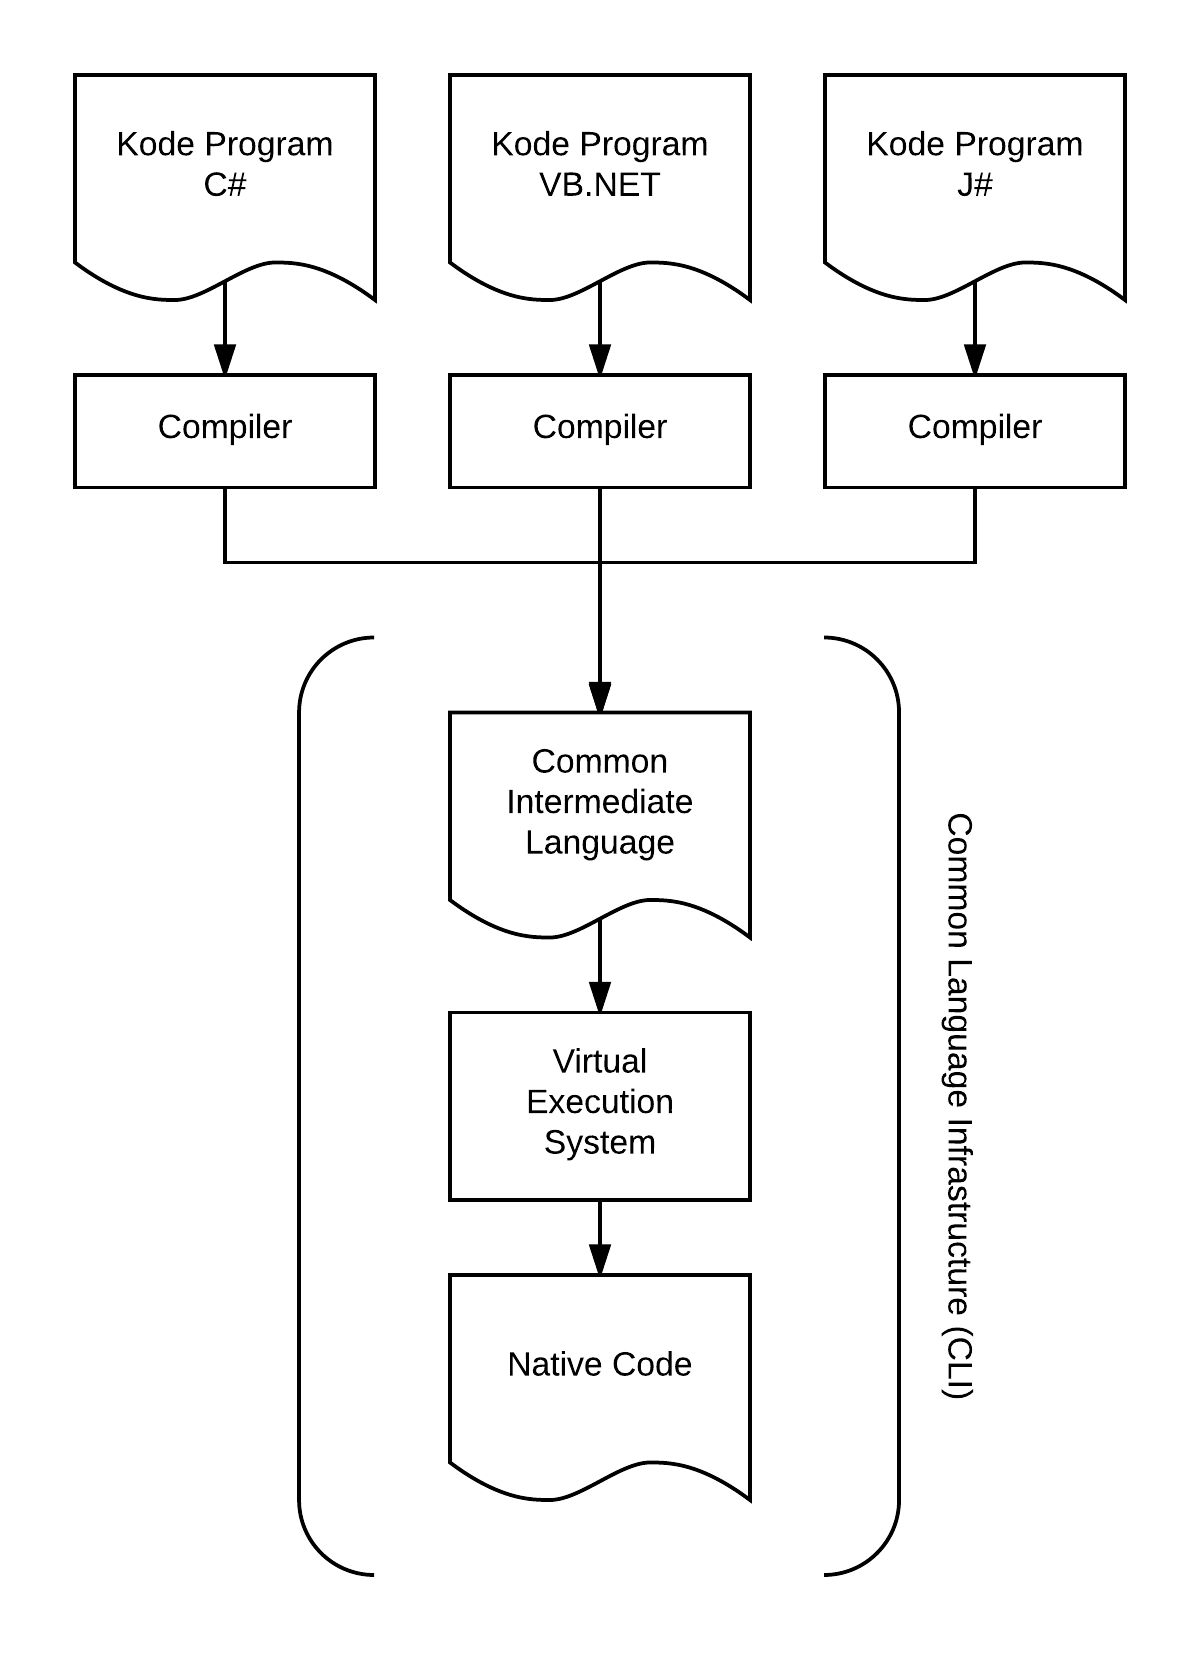
\includegraphics[scale=0.2]{Gambar/CLI.png}
    \caption[Diagram alir proses yang dilalui oleh kode program dalam CLI.]{Diagram alir proses yang dilalui oleh kode program dalam CLI.} 
    \label{fig:cli}
\end{figure}

Komponen-komponen penting dalam CLI di antaranya adalah\cite{CLI:2016}:

\begin{itemize}
    \item{\textit{Common Type System} (CTS)\\CTS memberikan \textit{type system} yang kaya dan mendukung tipe dan operasi yang ditemukan pada banyak bahasa pemrograman.}
    \item{\textit{Metadata}\\CLI menggunakan \textit{metadata} untuk menjelaskan dan mereferensi tipe-tipe yang didefinisikan oleh CTS.}
    \item{\textit{Common Language Spesification} (CLS)\\CLS adalah perjanjian desainer bahasa pemrograman dan desainer \textit{framework}. Perjanjian ini menentukan bagian minimal dari CTS yang harus diimplementasikan oleh bahasa pemrograman dan \textit{framework} yang bersangkutan.}
    \item{\textit{Virtual Execution System} (VES)\\VES mengimplementasikan model CTS dan memastikan hal tersebut berjalan sebagaimana mestinya. VES berfungsi untuk menjalankan program yang ditulis untuk CLI.}
\end{itemize}

Seperti yang dijelaskan pada Gambar \ref{fig:cli}, beberapa bahasa pemrograman yang kompatibel dengan .NET adalah C\#, VB.NET, dan J\#\cite{NET_PRIMER:2016}. Setelah kode program dari bahasa-bahasa tersebut diterjemahkan oleh \textit{compiler}nya masing-masing, maka akan terbentuk \textit{Common Intermediate Language} (CIL) yang kemudian akan dibaca dan dieksekusi oleh VES\cite{CLI:2016}. Implementasi VES pada .NET bernama \textit{Common Language Runtime} (CLR).



\section{\textit{Universal Windows Platform} (UWP)}
\label{sec:uwp}

Windows 8 memperkenalkan \textit{Windows Runtime} (WinRT) yang merupakan arsitektur aplikasi umum untuk Windows\cite{UWP:2016}. Saat Windows Phone 8.1 keluar, Windows Runtime pada Windows 8 dan Windows Phone 8.1 disejajarkan agar \textit{developer} dapat membangun satu aplikasi yang dapat dijalankan pada Windows 8 dan Windows Phone 8.1. \textit{Universal Windows Platform} (UWP) pertama kali diperkenalkan pada Windows 10 sebagai perubahan dari model \textit{Windows Runtime}. UWP tidak hanya dapat memanggil API dari WinRT, namun juga API spesifik dari device yang bersangkutan (seperti Win32 dan .NET).



\section{Kelas WebView Pada UWP}
\label{sec:webview}

Kelas WebView pada UWP memungkinkan \textit{developer} untuk menampung konten HTML pada suatu aplikasi\cite{WinAPI:2016}. WebView tidak mendukung masukkan pengguna seperti \textit{key-down}, \textit{key-up}, dan \textit{pointer-pressed}. Oleh karena itu, dibutuhkan metode lain yang melibatkan InvokeScriptAsync dengan fungsi \textit{eval} javascript untuk menggunakan HTML \textit{event handler} dan fungsi window.external.notify untuk menangani event dari HTML pada aplikasi.

Beberapa \textit{property} yang dimiliki oleh WebView adalah:

\begin{itemize}
    \item{DocumentTitle\\Menyimpan \textit{title} dari dokumen yang sedang ditampilkan dalam bentuk String.}
    \item{BaseUri\\Menyimpan \textit{uri} dari dokumen yang sedang ditampilkan dalam bentuk Uri.}
\end{itemize}

Beberapa \textit{method} yang dimiliki oleh WebView adalah:

\begin{itemize}
    \item{InvokeScriptAsync(String scriptName, String[] arguments)\\Method ini digunakan untuk melakukan eksekusi script tertentu pada HTML dengan argumen yang diberikan dalam bentuk \textit{array of string}.}
    \item{Navigate(Uri source)\\Method ini digunakan untuk membuka URI tertentu.}
\end{itemize}

Salah satu \textit{event} yang dimiliki oleh kelas WebView adalah \textit{event} ScriptNotify. \textit{Event} ini berguna untuk menangkap hasil dari fungsi javascript window.external.notify.



\section{Kelas PasswordVault Pada Windows}
\label{sec:passwordvault}

Kelas PasswordVault merupakan komponen dari Windows Runtime API, dan bukan .NET\cite{WinAPI:2016}. Kelas ini merepresentasikan pengunci kredensial. Kredensial yang disimpan menggunakan kelas ini hanya dapat diakses oleh aplikasi atau \textit{service} yang bersangkutan. Beberapa \textit{method} yang dimiliki oleh kelas PasswordVault adalah:

\begin{itemize}
    \item{Add(PasswordCredential credential)\\\textit{Method} ini berfungsi untuk memasukkan kredensial.}
    \item{Retrieve(String resource, String userName)\\\textit{Method} ini berfungsi untuk mengambil kredensial yang tersimpan di dalam objek PasswordVault.}
    \item{Remove(PasswordCredential credential)\\\textit{Method} ini berfungsi untuk menghapus kredensial yang tersimpan di dalam objek PasswordVault.}
\end{itemize}

}{}
\ifdefstring{\vbabc}{1}{\chapter{Analisis}
\label{chap:analisis}

Bab ini menjelaskan mengenai analisis perangkat lunak sejenis, analisis cara penyimpanan informasi login, analisis cara menangkap informasi login, serta analisis perangkat lunak.



\section{Analisis Perangkat Lunak Sejenis}
\label{sec:perangkat_lunak_sejenis}

Perangkat lunak sejenis pada Windows belum dapat ditemukan pada saat penelitian ini dilakukan. Oleh karena itu, perangkat lunak atau aplikasi sejenis yang dianalisis adalah aplikasi yang diciptakan untuk sistem operasi Android. Aplikasi tersebut bernama \textit{WiFi Web Login}.


\subsubsection{Diagram Alir \textit{WiFi Web Login}}
\label{subsubsec:diagram_alir_wifi_web_login}

Langkah-langkah yang perlu ditempuh oleh aplikasi \textit{WiFi Web Login} dapat digambarkan oleh diagram alir.

\begin{figure}[h]
    \centering
    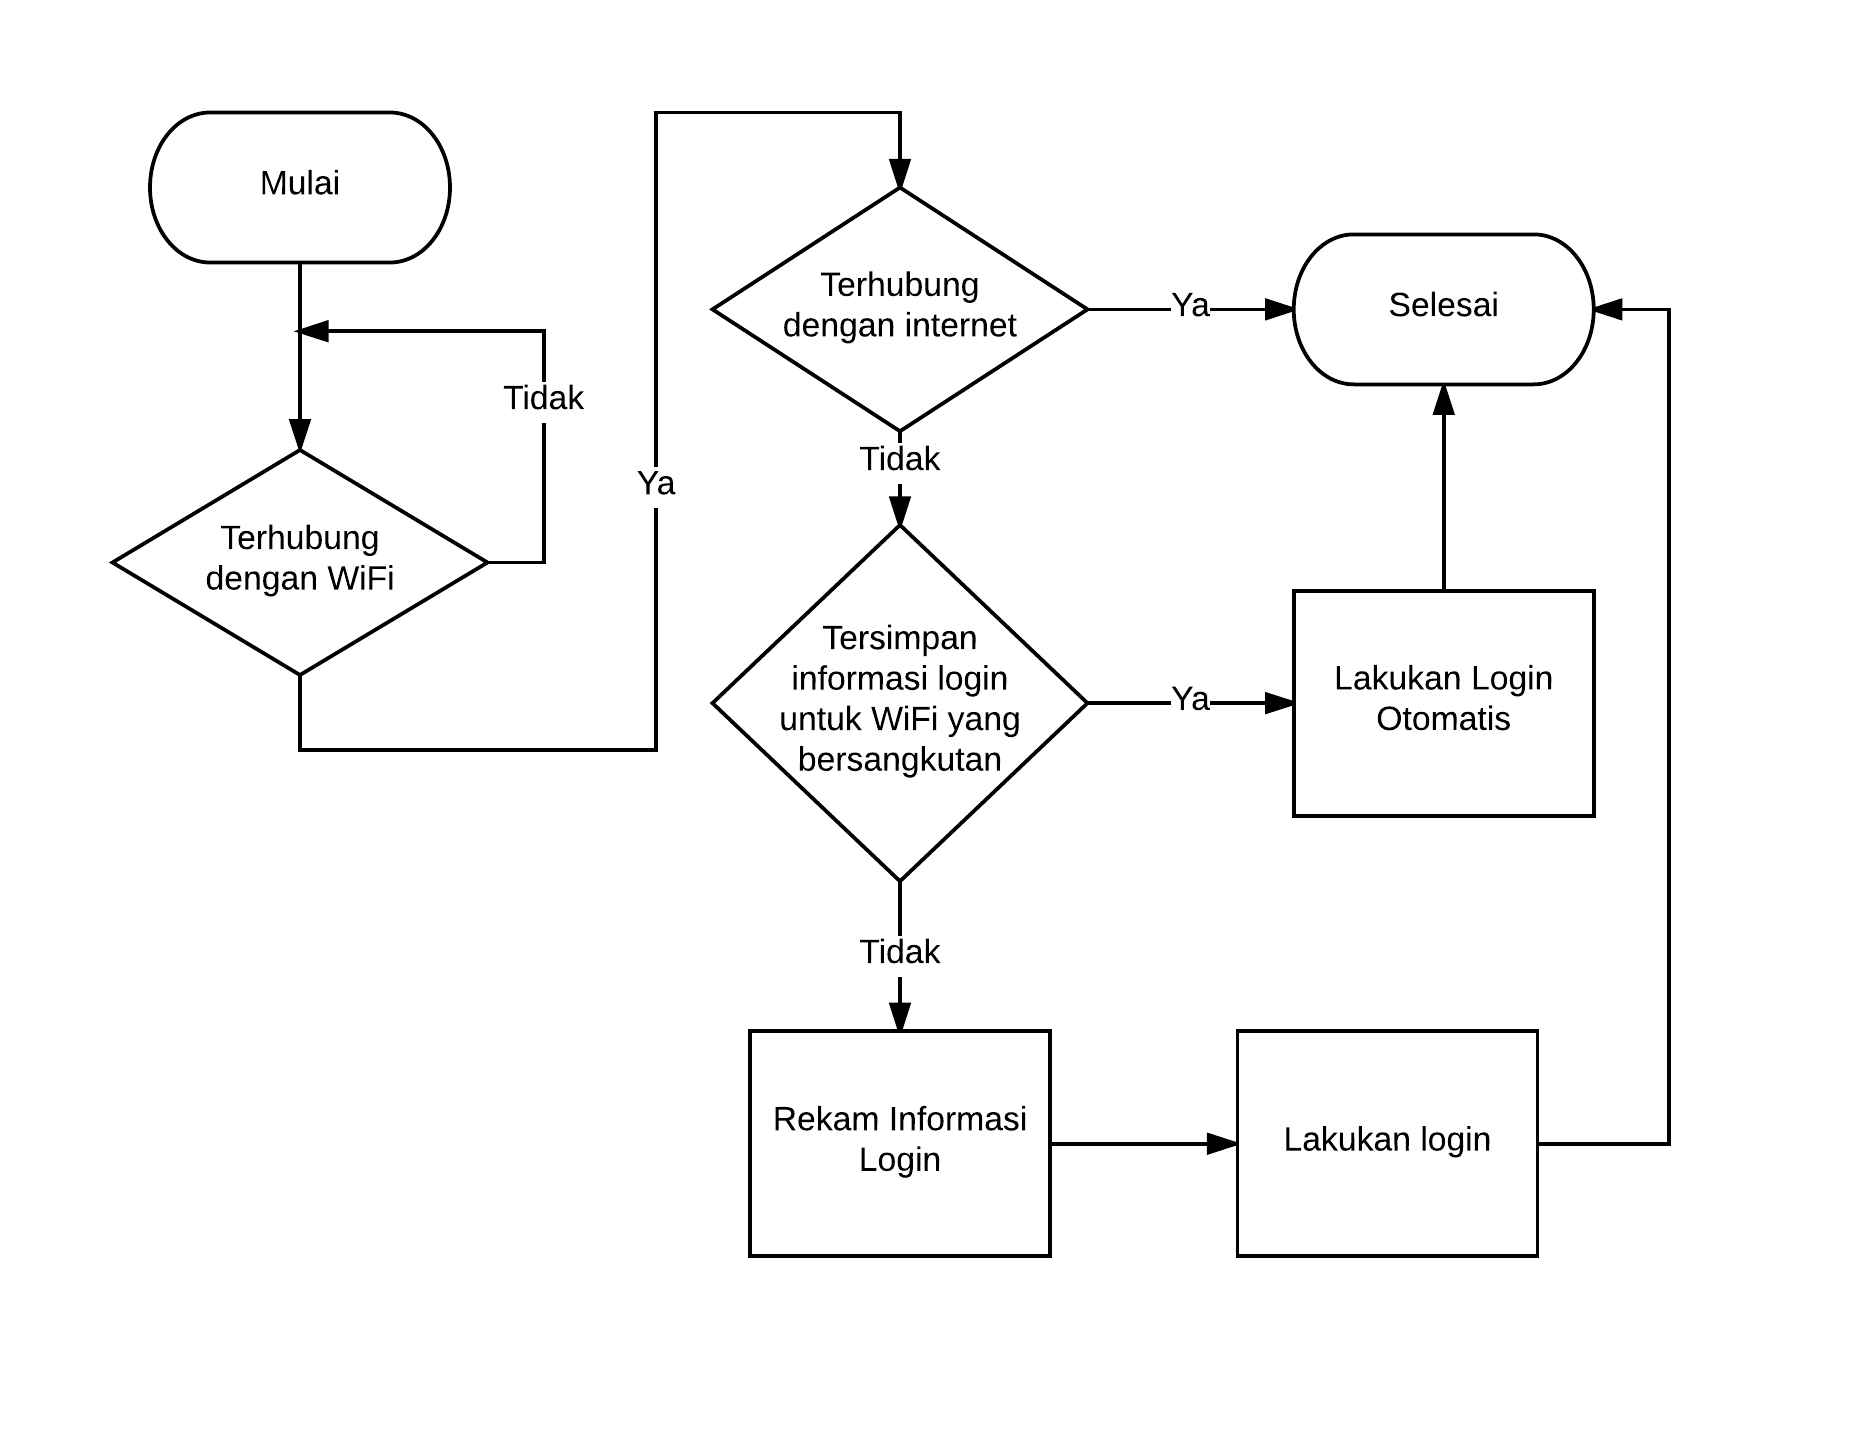
\includegraphics[scale=0.85]{Gambar/WifiWebLogin.png}
    \caption[Diagram alir proses yang perlu dilalui oleh aplikasi \textit{WiFi Web Login}.]{Diagram alir proses yang perlu dilalui oleh aplikasi \textit{WiFi Web Login}.} 
    \label{fig:wifiweblogin}
\end{figure}

Berdasarkan gambar \ref{fig:wifiweblogin}, langkah-langkah yang harus ditempuh untuk melakukan \textit{login} wifi berbasis web pada aplikasi ini adalah:

\begin{enumerate}
    \item{Deteksi sambungan dengan wifi yang bersangkutan.}
    \item{Deteksi hubungan dengan internet.}
    \item{Jika tidak terjadi hubungan dengan internet, deteksi apakah tersimpan informasi login untuk wifi yang bersangkutan.}
    \item{Jika terdapat informasi login untuk wifi yang bersangkutan maka lakukan login otomatis.}
    \item{Jika tidak terdapat informasi login untuk wifi yang bersangkutan maka rekam informasi login dan lakukan login.}
\end{enumerate}

Setelah pengguna melalui sudah pernah melakukan login pertama kali menggunakan aplikasi tersebut, maka aplikasi akan melakukan login otomatis setiap kali terhubung dengan wifi yang bersangkutan.



\section{Analisis Metode Penyimpanan Informasi Login}
\label{sec:metode_penyimpanan}

Penyimpanan informasi login dapat dilakukan dengan beberapa metode, diantaranya adalah dengan menggunakan file teks atau menggunakan \textit{credential locker}. Penyimpanan informasi menggunakan file teks berarti informasi disimpan dalam bentuk \textit{plaintext} dalam file yang diberikan \textit{access permission} tertentu. Sementara itu, penyimpanan informasi menggunakan credential locker memanfaatkan kelas PasswordVault yang terdapat pada \textit{Universal Windows Platform} (UWP).

Informasi yang perlu disimpan untuk dapat melakukan login otomatis adalah \textit{connection fingerprint} (seperti SSID WiFi, url, dan potongan unik dokumen html), username, password, dan langkah-langkah login seperti menekan tombol. Oleh karena itu, metode penyimpanan menggunakan credential locker dan file teks dianalisis untuk dapat ditentukan metode mana yang paling cocok untuk digunakan dalam penelitian ini.

\subsection{Credential Locker}
\label{subsec:credential_locker}

Credential locker dapat menyimpan informasi yang berisi \textit{resource} (biasanya berupa nama aplikasi atau string unik lainnya), username, dan password. Informasi yang perlu disimpan selain username dan password adalah \textit{connection fingerprint} dan langkah-langkah login. \textit{Connection fingerprint} dapat disimpan pada resource karena sifatnya yang unik, dan langkah-langkah login dapat disisipkan ke dalam field password dalam bentuk string dengan separator tertentu. Langkah-langkah login disisipkan ke dalam field password karena resource dan username adalah identifier yang dibutuhkan untuk melakukan retrieval informasi.

\textit{Credential locker} memiliki batasan 10 kredensial yang dapat disimpan per aplikasi. Jika aplikasi mencoba menyimpan lebih dari 10 kredensial maka akan terjadi exception. Oleh karena hal ini, \textit{credential locker} menjadi pilihan yang kurang baik untuk kebutuhan perangkat lunak pada penelitian ini.

\subsection{File Teks}
\label{subsec:file_teks}

Penyimpanan informasi mengunakan file teks dapat dilakukan untuk informasi berbasis teks apapun dan tidak ada batasan banyaknya informasi yang dapat disimpan (kecuali batasan perangkat keras seperti kapasitas hard disk). Akan tetapi, file teks dapat dibaca oleh aplikasi manapun, sehingga penyimpanan informasi sensitif seperti username dan password tidak dapat dilakukan tanpa adanya metode untuk memastikan hanya aplikasi bersangkutan yang dapat membacanya.

Salah satu metode pengamanan yang dapat dilakukan adalah dengan mendeklarasikan \textit{file access permission}. Akan tetapi, karena Windows memiliki \textit{security model} per pengguna dan bukan per aplikasi, maka aplikasi lain yang dijalankan oleh pengguna tersebut memiliki akses yang sama kepada file yang bersangkutan.

Model pengamanan lainnya adalah dengan melakukan enkripsi pada file yang bersangkutan sehingga hanya pemegang kunci yang dapat membaca file tersebut. Enkripsi file pada windows dapat dilakukan menggunakan kelas CryptographicEngine. Kunci enkripsi dan dekripsi dapat disimpan menggunakan \textit{credential locker} atau dengan meminta pengguna untuk memasukkan kunci tersebut setiap kali aplikasi dijalankan.



\section{Analisis Metode Rekam dan Kirim Informasi Login}
\label{sec:metode_rekam}

Kelas WebView pada \textit{Universal Windows Platform} (UWP) hanya dapat dihubungkan dengan kode C\# menggunakan javascript. \textit{Method} yang digunakan untuk melakukan eksekusi javascript pada WebView adalah InvokeScriptAsync. Metode ini memiliki parameter string berupa nama fungsi javascript yang ingin dipanggil dan array of string yang berisi argumen yang ingin dikirimkan ke dalam fungsi tersebut. Salah satu fungsi yang dapat dipanggil adalah \textit{eval}. Dengan menggunakan \textit{eval}, ekspresi javascript apapun dapat dijalankan pada WebView. Untuk mengirimkan data dari javascript ke kode C\#, dapat dijalankan fungsi window.external.notify dengan parameter berupa string. Oleh karena itu, diperlukan \textit{encoding} tertentu (seperti JSON) untuk memasukkan lebih dari satu argumen.

InvokeScriptAsync dapat digunakan untuk memanggil fungsi \textit{eval} dengan parameter berupa function yang dapat digunakan untuk menekan tombol atau memasukkan nilai pada \textit{text field} tertentu. Selain itu, dapat dimasukkan event listener yang dapat memanggil window.external.notify menggunakan cara ini. Fungsi window.external.notify dapat membantu mengirimkan event-event seperti mouse click, keypress, atau perubahan nilai pada \textit{text field} yang ada pada halaman HTML pada WebView tersebut.}{}
\ifdefstring{\vbabd}{1}{\chapter{Perancangan}
\label{chap:perancangan}

Bab ini menjelaskan mengenai perancangan yang disusun dari analisis yang dilakukan pada bab 3. Perancangan yang dilakukan mencakupi perancangan kelas, diagram \textit{sequence}, serta penjelasan mengenai hasil analisis yang tidak mungkin diimplementasikan dan cara lain yang dilakukan untuk mendapatkan hasil yang serupa.



\section{Perancangan Kelas}
\label{sec:perancangan_kelas}

Gambar \ref{fig:DetailedClassDiagram} menjelaskan mengenai kelas-kelas dalam perangkat lunak yang dibuat. Beberapa kelas utama yang perlu dijelaskan antara lain:

\par{\textbf{MainPage} : Kelas ini merupakan kelas yang berperan sebagai tampilan utama aplikasi. Atribut-atribut yang dimiliki oleh kelas ini adalah:
    \begin{itemize}
        \item{cpd\\Atribut untuk menyimpan \textit{instance} CaptivePortalDetector.}
        \item{timeoutTimer\\Atribut untuk menyimpan timer yang digunakan untuk menghitung \textit{connection timeout}.}
        \item{loaded\\Atribut untuk menyimpan status \textit{loading} suatu halaman.}
    \end{itemize}
    Metode-metode yang dimiliki oleh kelas ini adalah:
    \begin{itemize}
        \item{setup\\Metode ini digunakan untuk melakukan \textit{setup} awal saat aplikasi dieksekusi. Fungsinya adalah untuk menyimpan \textit{instance} CaptivePortalDetector dan memanggil metode setup() pada \textit{instance} tersebut.}
        \item{MainWebView\_LoadCompleted\\Metode ini dipanggil saat WebView selesai melakukan loading halaman. Fungsinya adalah untuk memanggil metode onLoad() pada CaptivePortalDetector.}
        \item{MainWebView\_NavigationStarting\\Metode ini dipanggil saat WebView baru akan memulai navigasi ke halaman baru. Fungsinya adalah untuk memulai \textit{timer} untuk \textit{timeout} dan memasukkan objek ScriptNotifyHandler.}
        \item{MainWebView\_NewWindowRequested\\Metode ini dipanggil saat WebView melakukan \textit{request} untuk membuka window baru. Fungsinya adalah untuk memanggil metode queueUri() pada CaptivePortalDetector.}
        \item{MainWebView\_NavigationCompleted\\Metode ini dipanggil saat WebView selesai melakukan navigasi ke halaman baru, namun belum selesai melakukan loading halaman tersebut. Fungsinya adalah untuk melakukan \textit{override} fungsi-fungsi JavaScript seperti window.open() dan open() agar bisa diakses dari JavaScript tanpa aksi langsung dari pengguna.}
    \end{itemize}
}

\begin{figure}[!htb]
    \centering
    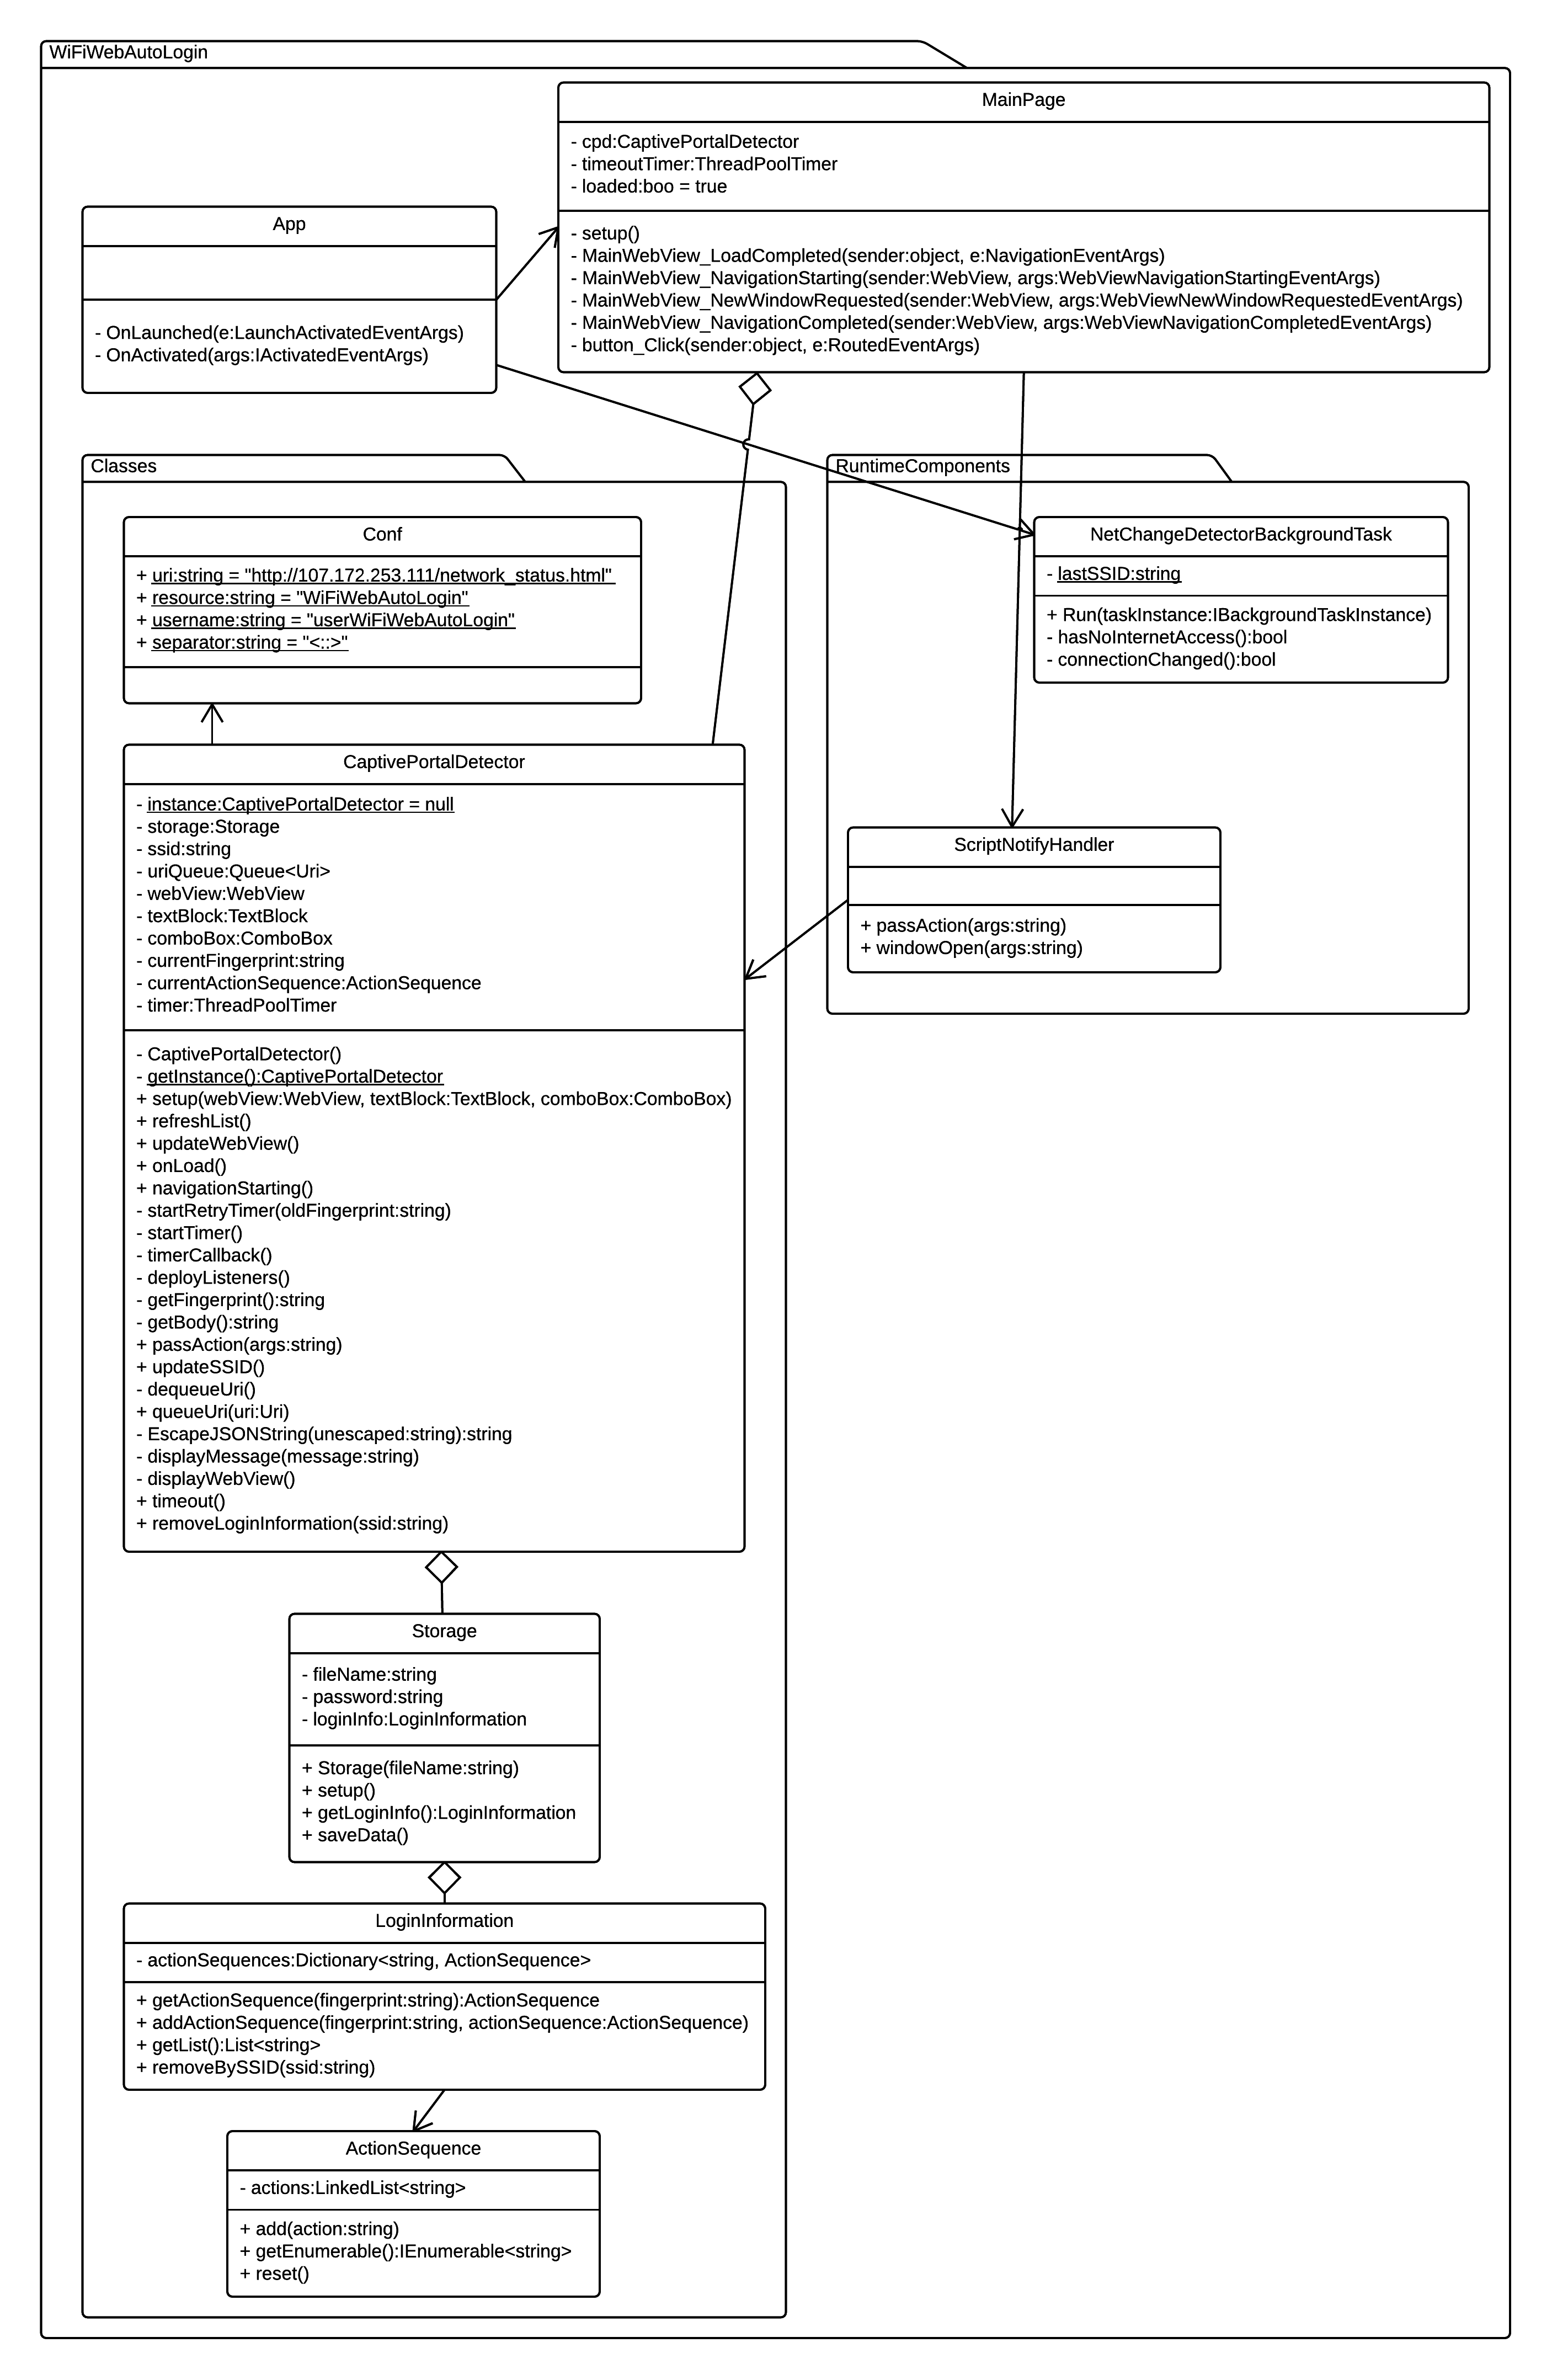
\includegraphics[scale=0.63]{Gambar/DetailedClassDiagram.png}
    \caption[Diagram Kelas Rinci.]{Diagram Kelas Rinci.} 
    \label{fig:DetailedClassDiagram}
\end{figure}

\par{\textbf{NetChangeDetectorBackgroundTask} : Kelas ini merupakan kelas yang digunakan untuk melakukan deteksi perubahan jaringan yang nantinya digunakan untuk menampilkan notifikasi apabila terdeteksi adanya jaringan yang terhubung tanpa adanya internet. Atribut yang dimiliki oleh kelas ini adalah:
    \begin{itemize}
        \item{lastSSID\\Atribut ini menyimpan SSID terakhir yang nantinya akan dibandingkan dengan SSID terbaru untuk mendeteksi adanya perubahan SSID.}
    \end{itemize}
    Metode-metode yang dimiliki oleh kelas ini adalah:
    \begin{itemize}
        \item{Run\\Metode ini dipanggil saat Windows mengalami perubahan jaringan. Fungsinya adalah untuk menampilkan notifikasi apabila kondisi \texttt{connectionChanged()}, \texttt{lastSSID!=null}, dan \texttt{hasNoInternetAccess()} terpenuhi.}
        \item{hasNoInternetAccess\\Metode ini digunakan untuk medeteksi tidak adanya akses internet menggunakan API yang diberkan oleh UWP.}
        \item{conectionChanged\\Metode ini digunakan untuk medeteksi perubahan SSID.}
    \end{itemize}
}

\par{\textbf{ScriptNotifyHandler} : Kelas ini merupakan kelas yang digunakan untuk menghubungkan sisi javascript pada WebView dengan kode C\#. Metode-metode yang dimiliki oleh kelas ini adalah:
    \begin{itemize}
        \item{passAction\\Metode ini dipanggil saat \textit{listener} yang sudah disisipkan ke dalam WebView mendeteksi \textit{action} yang dapat direkam. \textit{Action} yang direkam berupa teks yang berisi kode javascript yang dapat mereplikasi \textit{action} tersebut.}
        \item{windowOpen\\Metode ini dipanggil saat javascript pada WebView memanggil fungsi window.open atau fungsi open.}
    \end{itemize}
}

\par{\textbf{CaptivePortalDetector} : Kelas ini merupakan kelas utama yang berfungsi untuk melakukan deteksi \textit{captive portal}, menyisipkan kode \textit{listener} pada WebView, merekam \textit{action sequence} yang dilakukan oleh pengguna, dan menjalankan kembali \textit{action sequence} yang sudah tersimpan. Kelas ini menggunakan \textit{design pattern} singleton agar kelas-kelas lainnya bisa mengakses \textit{instance} yang sama pada setiap \textit{session}. Atribut yang dimiliki oleh kelas ini adalah:
    \begin{itemize}
        \item{instance\\Atribut ini menyimpan \textit{instance} CaptivePortalDetector.}
        \item{storage\\Atribut ini menyimpan objek Storage yang digunakan untuk menyimpan dan mengakses informasi login.}
        \item{ssid\\Atribut ini menyimpan SSID saat ini.}
        \item{uriQueue\\Atribut ini menyimpan queue Uri yang perlu diakses.}
        \item{webView\\Atribut ini menyimpan WebView yang digunakan untuk melakukan deteksi \textit{captive portal}.}
        \item{textBlock\\Atribut ini menyimpan TextBlock yang digunakan untuk menampilkan pesan kepada pengguna.}
        \item{comboBox\\Atribut ini menyimpan ComboBox yang digunakan untuk menampilkan daftar SSID yang sudah tersimpan kepada pengguna.}
        \item{currentFingerprint\\Atribut ini menyimpan fingerprint saat ini.}
        \item{currentActionSequence\\Atribut ini menyimpan ActionSequence yang terkait dengan fingerprint saat ini.}
        \item{timer\\Atribut ini menyimpan timer yang digunakan untuk mengatur waktu akses Uri dalam uriQueue.}
    \end{itemize}
    Metode-metode yang dimiliki oleh kelas ini adalah:
    \begin{itemize}
        \item{getInstance\\Metode ini digunakan untuk mendapatkan \textit{instance} dari CaptivePortalDetector.}
        \item{setup\\Metode ini digunakan untuk melakukan \textit{setup} awal yang menyimpan WebView, TextBlock, dan ComboBox ke dalam \textit{instance} CaptivePortalDetector.}
        \item{refreshList\\Metode ini digunakan untuk melakukan \textit{refresh} tampilan ComboBox.}
        \item{updateWebView\\Metode ini digunakan untuk menentukan melakukan deteksi \textit{captive portal} jika terhubung dengan koneksi WiFi, atau menampilkan pesan kepada pengguna juka tidak terhubung dengan koneksi WiFi.}
        \item{onLoad\\Metode ini dipanggil saat WebView sudah selesai melakukan \textit{loading} halaman. Fungsinya adalah untuk melakukan deployListener(), menjalankan aksi-aksi yang sudah terekam pada informasi login, dan mendeteksi sudah atau belum terjadinya koneksi dengan internet.}
        \item{navigationStarting\\Metode ini dipanggil saat WebView mulai melakukan navigasi ke halaman baru. Fungsinya adalah untuk membatalkan timer untuk membuka halaman-halaman popup dari halaman sebelumnya.}
        \item{passAction\\Metode ini digunakan untuk menyimpan \textit{action} yang dikirimkan oleh ScriptNotifyHandler ke dalam currentActionSequence.}
        \item{updateSSID\\Metode ini digunakan untuk mendapatkan SSID terbaru.}
        \item{queueUri\\Metode ini digunakan untuk memasukkan Uri baru ke dalam uriQueue.}
        \item{timeout\\Metode ini digunakan untuk menyatakan bahwa terjadi \textit{connection timeout}.}
        \item{removeLoginInformation\\Metode ini digunakan untuk menghapus seluruh informasi login yang terkait dengan SSID tertentu.}
    \end{itemize}
}

\par{\textbf{Storage} : Kelas ini digunakan untuk menyimpan informasi login dan password yang digunakan untuk melakukan enkripsi. Atribut yang dimiliki oleh kelas ini adalah:
    \begin{itemize}
        \item{fileName\\Atribut ini menyimpan nama file yang digunakan untuk menyimpan informasi login yang terenkripsi.}
        \item{password\\Atribut ini menyimpan password yang digunakan untuk melakukan enkripsi.}
        \item{loginInfo\\Atribut ini menyimpan objek LoginInformation yang digunakan untuk menyimpan seluruh informasi login.}
    \end{itemize}
    Metode-metode yang dimiliki oleh kelas ini adalah:
    \begin{itemize}
        \item{setup\\Metode ini digunakan untuk melakukan \textit{setup} awal seperti membuka file dan melakukan dekripsi.}
        \item{getLoginInfo\\Metode ini digunakan untuk mendapatkan objek LoginInformation.}
        \item{saveData\\Metode ini digunakan untuk menyimpan data yang ada pada objek LoginInformation ke dalam file dan melakukan enkripsi pada file tersebut.}
    \end{itemize}
}

\par{\textbf{LoginInformation} : Kelas ini digunakan untuk merepresentasikan informasi login. Atribut yang dimiliki oleh kelas ini adalah:
    \begin{itemize}
        \item{actionSequences\\Atribut ini merupakan pasangan \textit{key-value} antara suatu fingerprint dengan ActionSequence.}
    \end{itemize}
    Metode-metode yang dimiliki oleh kelas ini adalah:
    \begin{itemize}
        \item{getActionSequence\\Metode ini digunakan untuk mendapatkan ActionSequence berdasarkan fingerprint tertentu.}
        \item{addActionSequence\\Metode ini digunakan untuk menambahkan ActionSequence untuk fingerprint tertentu.}
        \item{removeBySSID\\Metode ini digunakan untuk menghapus ActionSequence milik fingerprint tertentu.}
        \item{getList\\Metode ini digunakan untuk mendapatkan daftar SSID yang sudah direkam.}
    \end{itemize}
}

\par{\textbf{ActionSequence} : Kelas ini digunakan untuk merepresentasikan urutan \textit{action}. Atribut yang dimiliki oleh kelas ini adalah:
    \begin{itemize}
        \item{actions\\Atribut ini merupakan daftar \textit{action} yang berupa kode javascript.}
    \end{itemize}
    Metode-metode yang dimiliki oleh kelas ini adalah:
    \begin{itemize}
        \item{add\\Metode ini digunakan untuk menambahkan \textit{action} ke dalam daftar ini.}
        \item{getEnumerable\\Metode ini digunakan untuk mendapatkan enumerable dari daftar \textit{actions}, sehingga mempermudah eksekusi \textit{actions}.}
        \item{reset\\Metode ini digunakan untuk menghapus seluruh \textit{action} yang ada pada daftar ini.}
    \end{itemize}
}



\section{Perancangan Algoritma dan Struktur Data}
\label{sec:perancangan_algoritma_dan_struktur_data}

Sub-bab ini menjelaskan mengenai perancangan algoritma untuk melakukan deteksi \textit{captive portal}, struktur data dan format \textit{fingerprint}, serta struktur data untuk menyimpan informasi login.

\subsection{Algoritma Deteksi \textit{Captive Portal}}
\label{subsec:algoritma_deteksi_captive_portal}

Algoritma yang digunakan untuk melakukan deteksi \textit{captive portal} adalah sebagai berikut:

\hfill

\begin{algorithm}[H]
    \If{Network Detected and No Internet Connection}{
        Ask user to run application via notification\;
        \If{"Yes" button clicked}{
            Access a web page which can only be opened if there is an internet connection\;
            \If{Redirected}{
                Captive portal detected\;
            }
        }
    }
\end{algorithm}

\hfill

Algoritma di atas menjelaskan deteksi \textit{captive portal} dilakukan dengan melakukan deteksi jaringan yang tidak terhubung dengan internet. Jika ditemukan jaringan yang tidak terhubung dengan internet, maka akan muncul notifikasi yang memungkinkan pengguna untuk menjalankan perangkat lunak. Perangkat lunak akan mencoba untuk mengakses halaman pancingan yang beralamatkan pada \texttt{http://107.172.253.111/network\_status.html} pada saat perangkat lunak pertama kali dijalankan. Jika didapat respon HTTP yang berupa \textit{redirect}, maka pada jaringan tersebut terdapat \textit{captive portal}. Algoritma ini akan didaftarkan pada sistem saat perangkat lunak pertama kali dijalankan dan dipanggil saat ada perubahan status jaringan.

\subsection{Struktur Data dan Format \textit{Fingerprint}}
\label{subsec:struktur_data_dan_format_fingerprint}

\textit{Fingerprint} suatu halaman terdiri dari SSID, uri, serta isi \textit{tag} head pada halaman tersebut. Data ini disimpan dalam satu buah string dan dipisahkan oleh separator "<::>" (tanpa tanda petik). Salah satu contoh \textit{fingerprint} adalah:

\hfill

\texttt{UNPAR9<::>https://cas.unpar.ac.id/login<::><title>Halaman Login</title>}\\\\
yang memiliki arti bahwa \textit{fingerprint} tersebut berasal dari WiFi dengan:

\begin{itemize}
    \item{SSID \texttt{UNPAR9},}
    \item{uri \texttt{https://cas.unpar.ac.id/login},}
    \item{serta isi \textit{tag} head \texttt{<title>Halaman Login</title>}.}
\end{itemize}

\subsection{Struktur Data LoginInformation}
\label{subsec:struktur_data_logininformation}

Kelas LoginInformation memiliki daftar objek bertipe ActionSequence yang disimpan pada properti actionSequences bertipe Dictionary. Kelas Dictionary dapat menyimpan data yang berupa pasangan \textit{key-value}. \textit{Key} yang digunakan bertipe string dan merupakan \textit{fingerprint} suatu halaman. Value yang disimpan adalah objek bertipe ActionSequence yang merupakan list aksi-aksi yang perlu dilakukan untuk halaman tersebut.

Kelas ActionSequence memiliki properti actions yang bertipe LinkedList<string>. Setiap elemen LinkedList tersebut menyimpan string yang merupakan kode JavaScript yang akan dieksekusi pada halaman yang bersangkutan. \textit{Username} dan \textit{password} juga tersimpan di dalam kode JavaScript tersebut. Salah satu contoh string yang disimpan dalam properti actions adalah \texttt{document.getElementsByTagName("input")[0].value = "username";} yang berarti ubah isi elemen input pertama dengan "username".


\section{Perancangan Interaksi Perangkat Lunak}
\label{sec:perancangan_interaksi}

Beberapa interaksi yang dimodelkan menggunakan diagram interaksi adalah interaksi deteksi jaringan, interaksi penciptaan password, dan interaksi penyimpanan informasi login.

\subsection{Perancangan Interaksi Deteksi Jaringan}
\label{subsec:perancangan_interaksi_deteksi_jaringan}

\begin{figure}[!htb]
    \centering
    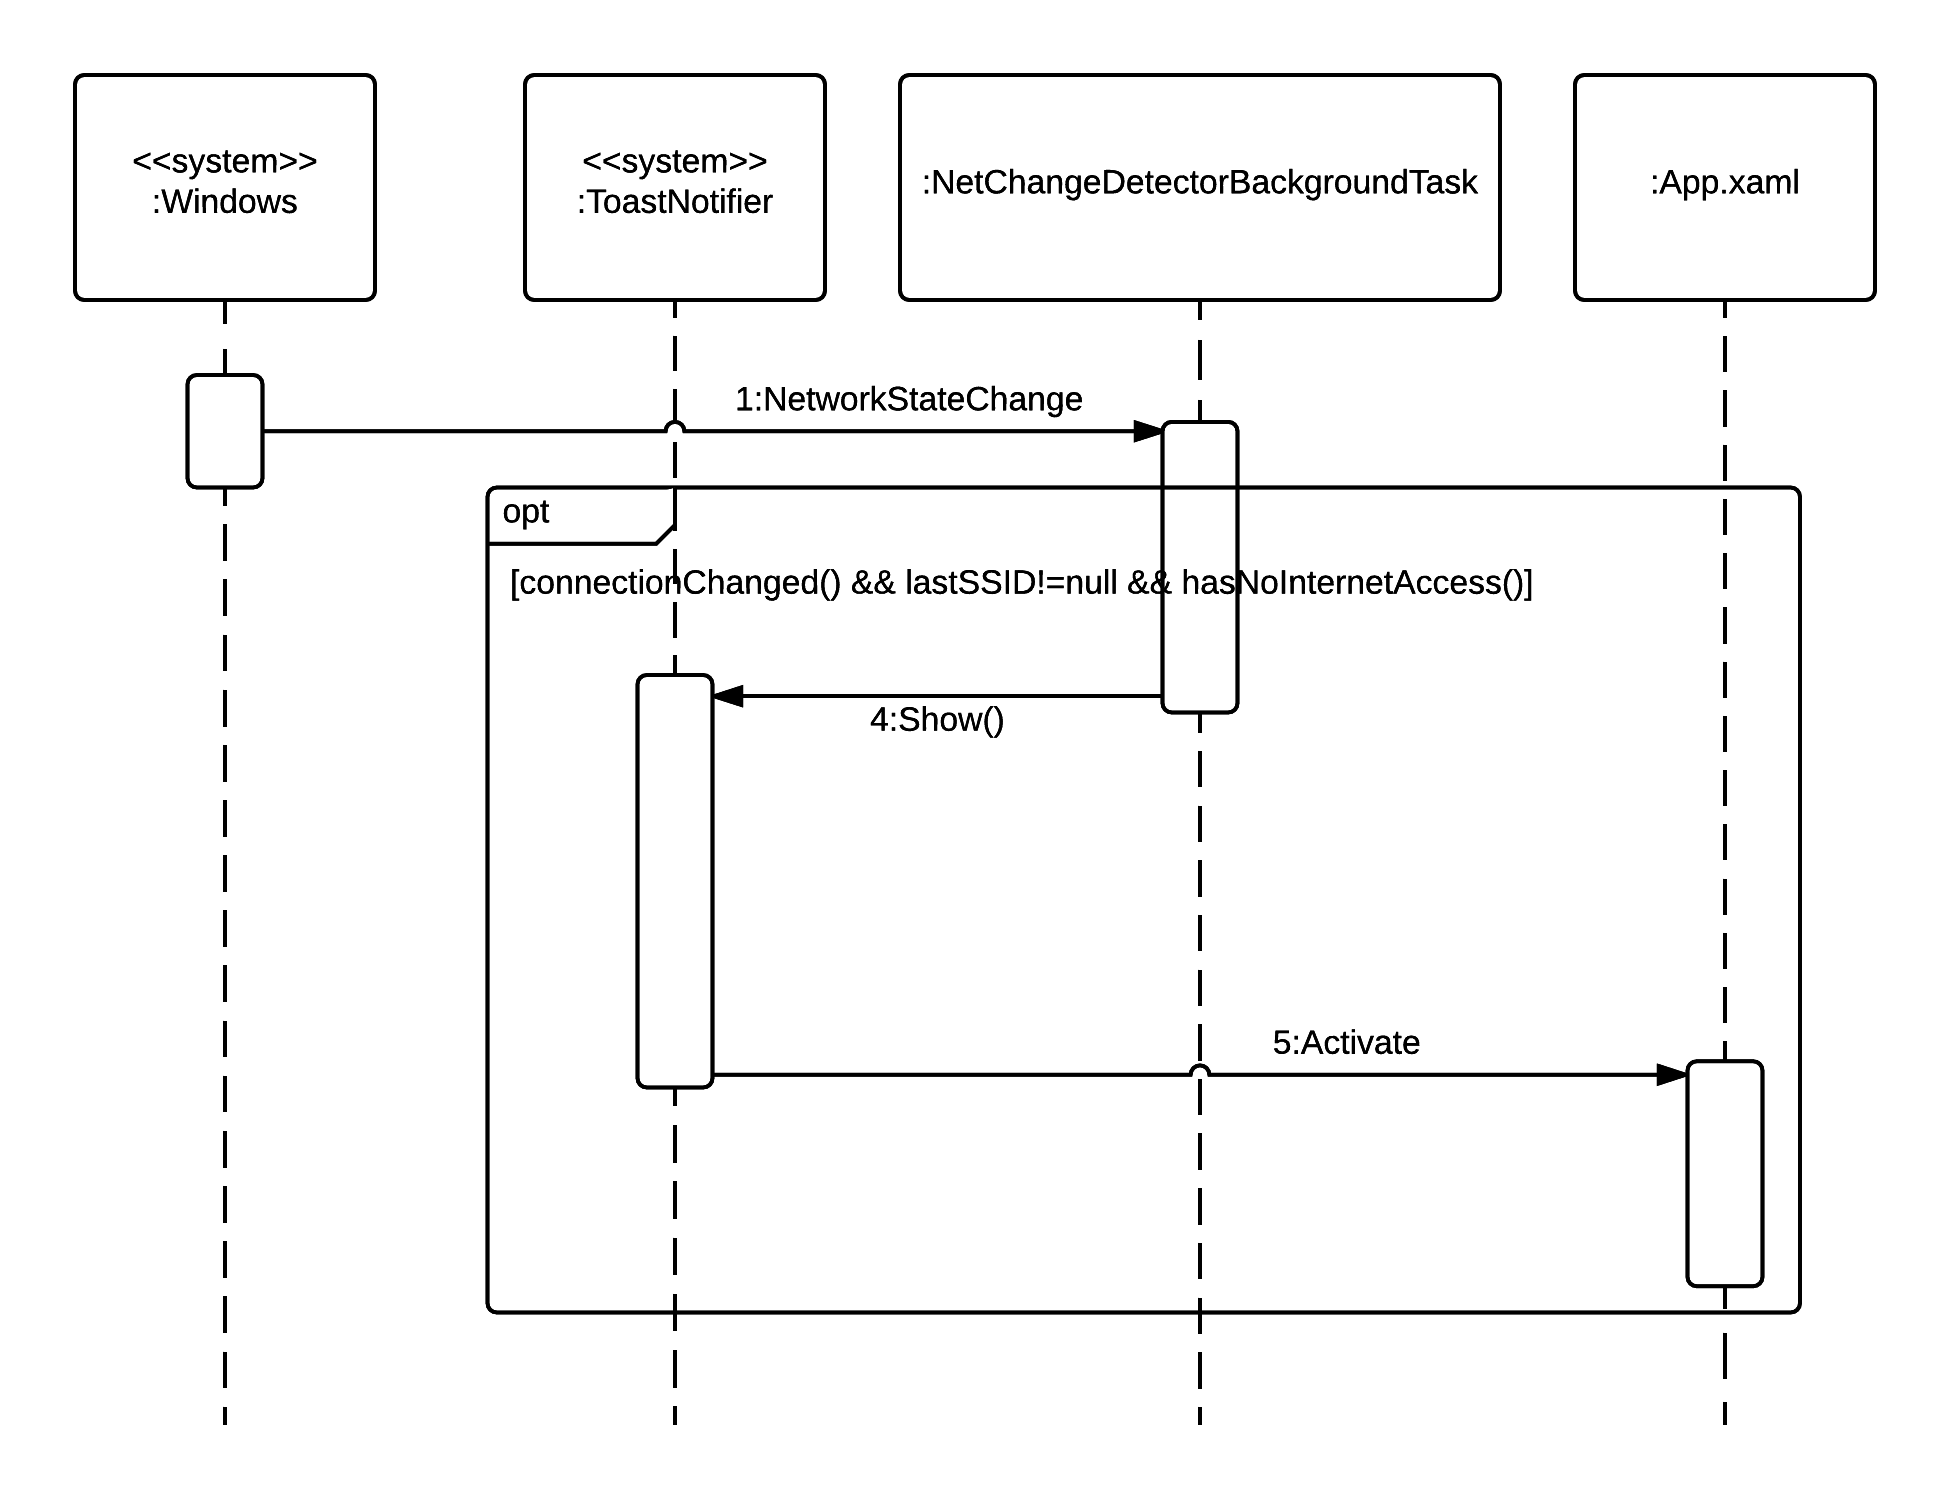
\includegraphics[scale=0.9]{Gambar/SequenceDiagramNetworkDetection.png}
    \caption[Diagram Interaksi Deteksi Jaringan.]{Diagram Interaksi Deteksi Jaringan.} 
    \label{fig:NetworkDetectionSequenceDiagram}
\end{figure}

Gambar \ref{fig:NetworkDetectionSequenceDiagram} menjelaskan mengenai interaksi antar objek dalam perangkat lunak untuk melakukan deteksi perubahan jaringan. Interaksi yang terjadi adalah sebagai berikut:

\begin{enumerate}
    \item{Saat komputer mengalami perubahan jaringan (tidak terhubung menjadi terhubung dan sebaliknya, atau terjadi perubahan \textit{cost} jaringan), \textit{trigger} NetworkStateChange akan diaktifkan oleh Windows, dan objek NetChangeDetectorBackgroundTask yang sudah didaftarkan akan menerima \textit{trigger} tersebut.}
    \item{Jika kondisi \texttt{connectionChanged()}, \texttt{lastSSID!=null}, dan \texttt{hasNoInternetAccess()} terpenuhi, maka:}
    \begin{enumerate}
        \item{NetChangeDetectorBackgroundTask memerintahkan ToastNotifier untuk memunculkan notifikasi menggunakan method Show().}
        \item{Saat user menekan tombol "Yes" pada notifikasi, App.xaml diaktivasi.}
    \end{enumerate}
\end{enumerate}

\subsection{Perancangan Interaksi Penciptaan Password}
\label{subsec:perancangan_interaksi_penciptaan_password}

\begin{figure}[!htb]
    \centering
    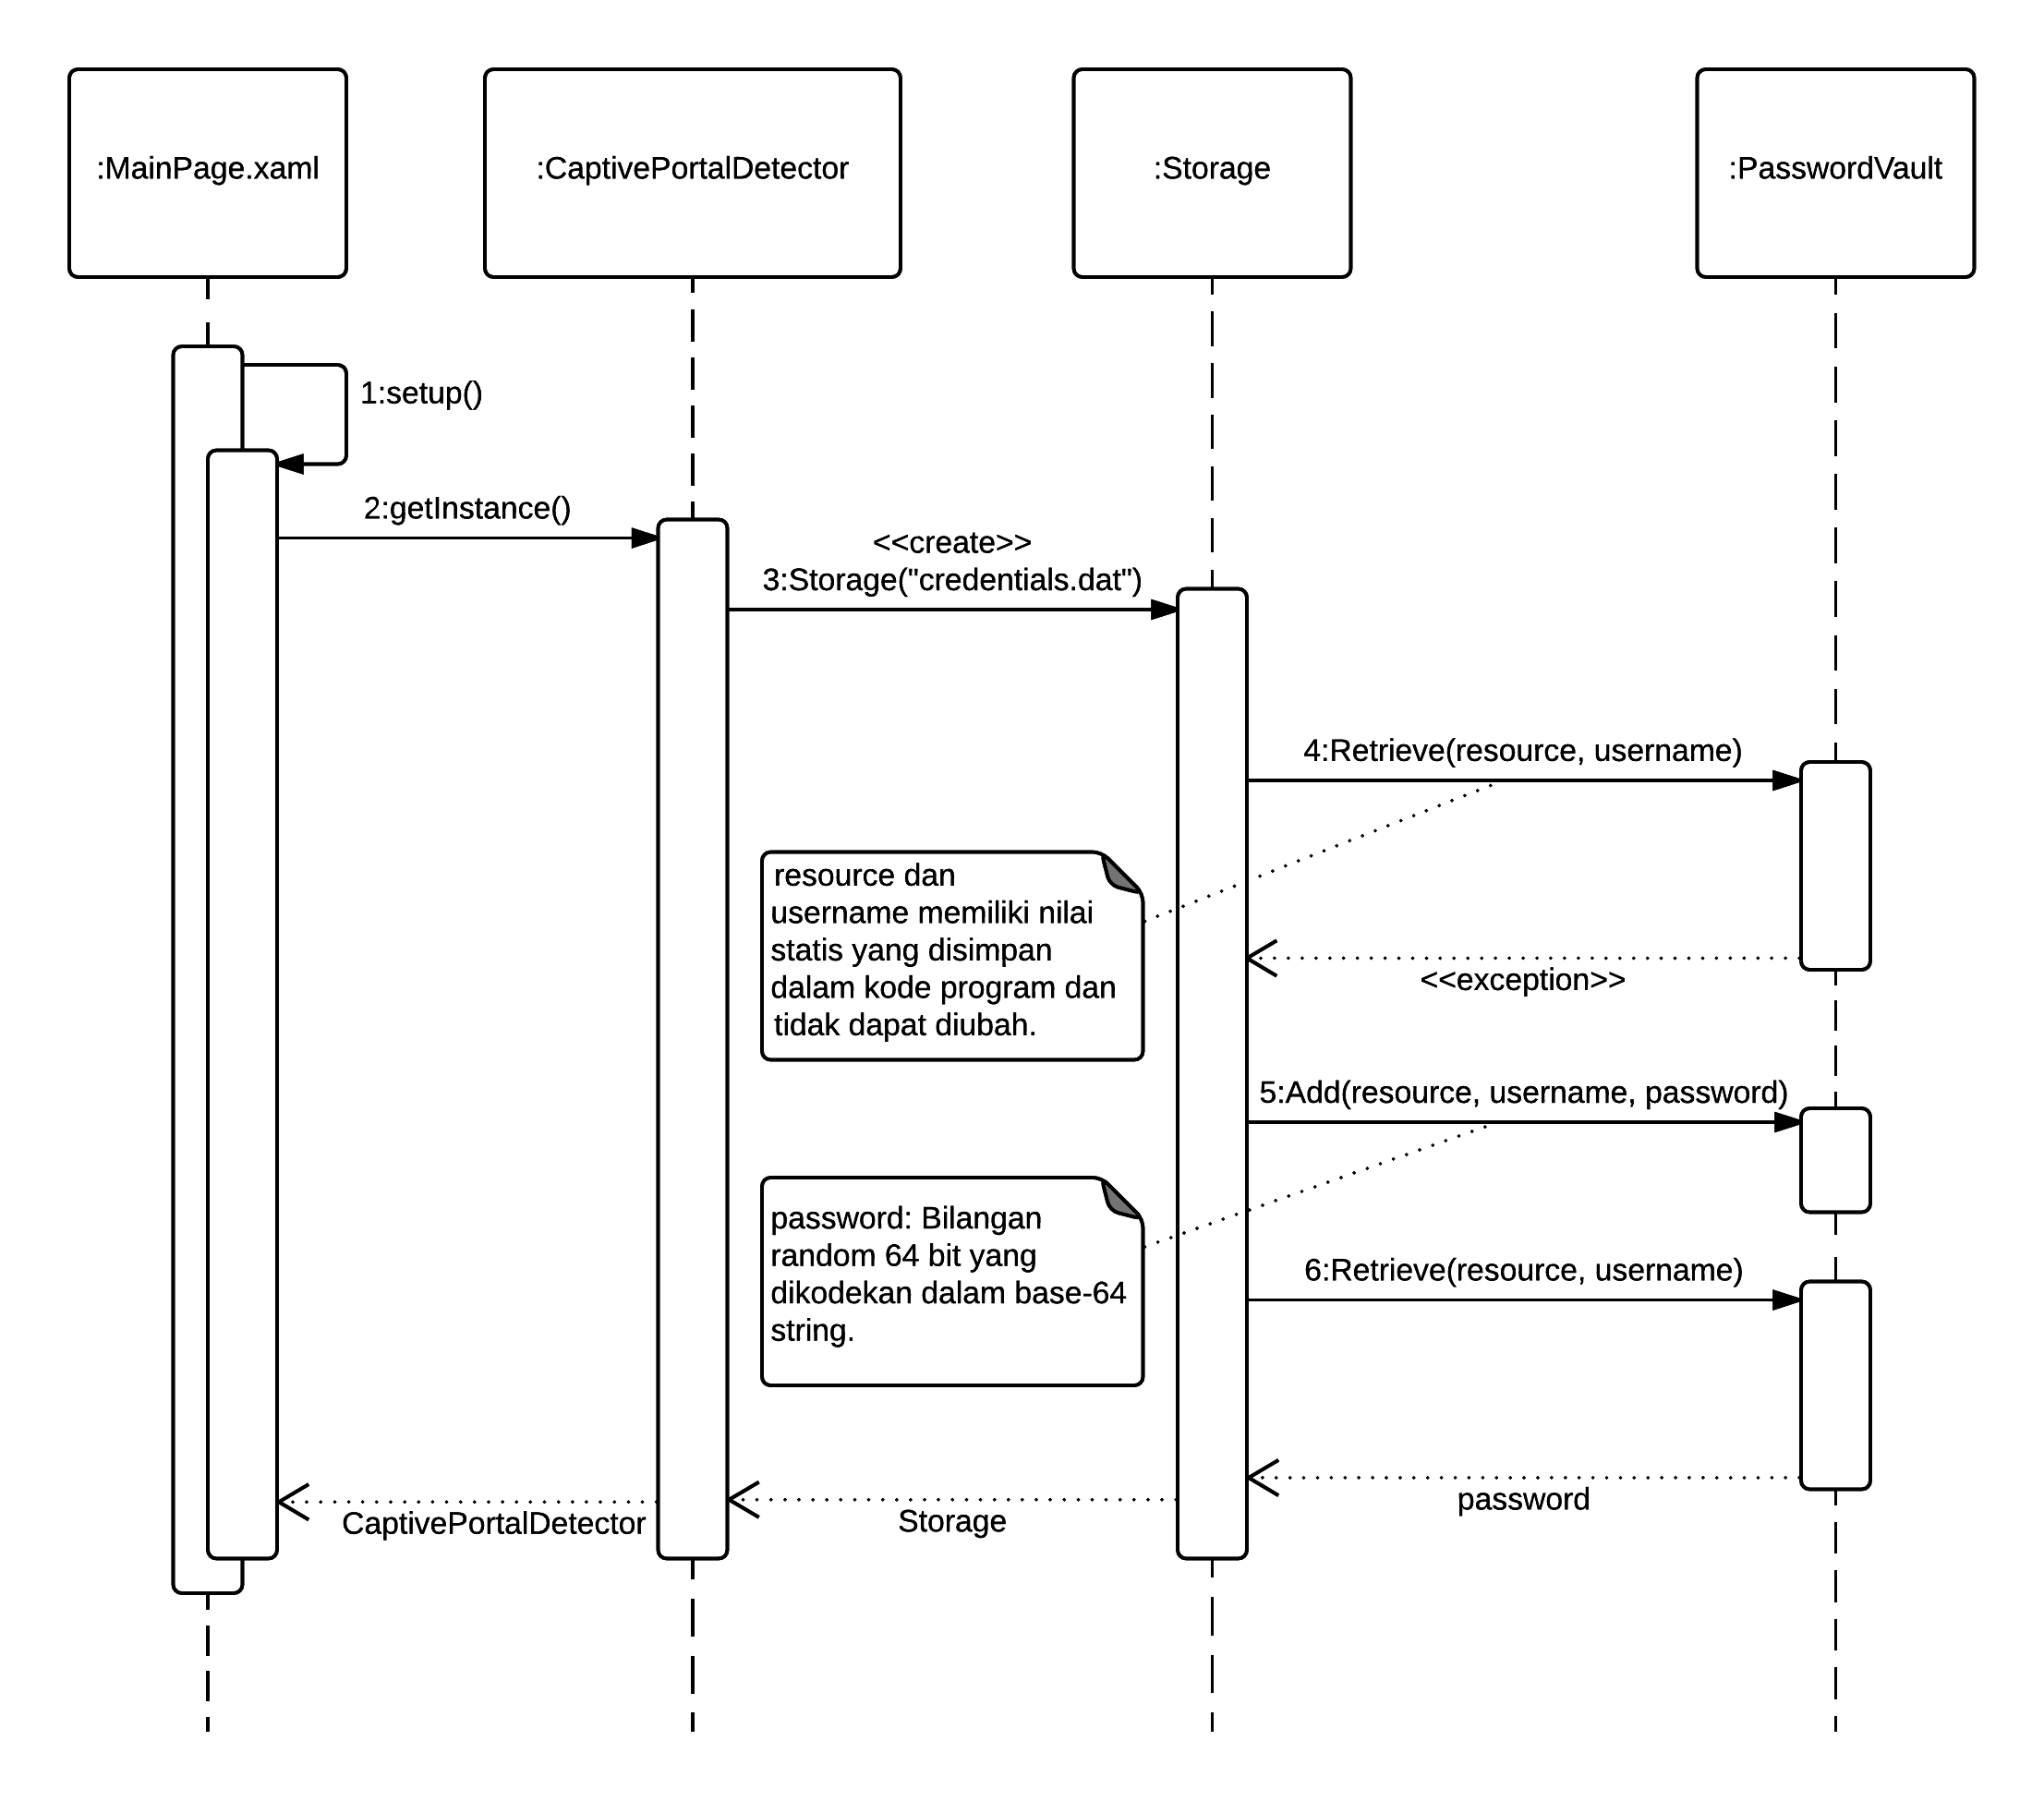
\includegraphics[scale=0.8]{Gambar/SequenceDiagramPasswordGeneration.png}
    \caption[Diagram Interaksi Penciptaan Password.]{Diagram Interaksi Penciptaan Password.} 
    \label{fig:PasswordGenerationSequenceDiagram}
\end{figure}

Gambar \ref{fig:PasswordGenerationSequenceDiagram} menjelaskan mengenai interaksi antar objek dalam perangkat lunak untuk menciptakan password random saat perangkat lunak pertama kali dijalankan. Interaksi yang terjadi adalah sebagai berikut:

\begin{enumerate}
    \item{MainPage.xaml melakukan setup().}
    \item{MainPage.xaml memanggil metode getInstance() pada CaptivePortalDetector untuk mendapatkan \textit{instance} CaptivePortalDetector.}
    \item{CaptivePortalDetector menciptakan objek Storage baru pada \textit{constructor}-nya.}
    \item{Objek Storage berusaha untuk mendapatkan password dengan memangil metode Retrieve() pada objek PasswordVault, namun mendapatkan exception karena belum ada password yang disimpan.}
    \item{Objek Storage memasukkan password baru yang diciptakan secara random menggunakan metode Add() pada PasswordVault.}
    \item{Objek Storage memanggil metode Retrieve() kembali pada objek PasswordVault, dan mendapatkan password yang baru saja diciptakan. Setelah itu, CaptivePortalDetector mendapatkan objek Storage, dan MainPage.xaml mendapatkan \textit{instance} CaptivePortalDetector.}
\end{enumerate}

\subsection{Perancangan Interaksi Penyimpanan Informasi Login}
\label{subsec:perancangan_interaksi_penciptaan_password}

\begin{figure}[!htb]
    \centering
    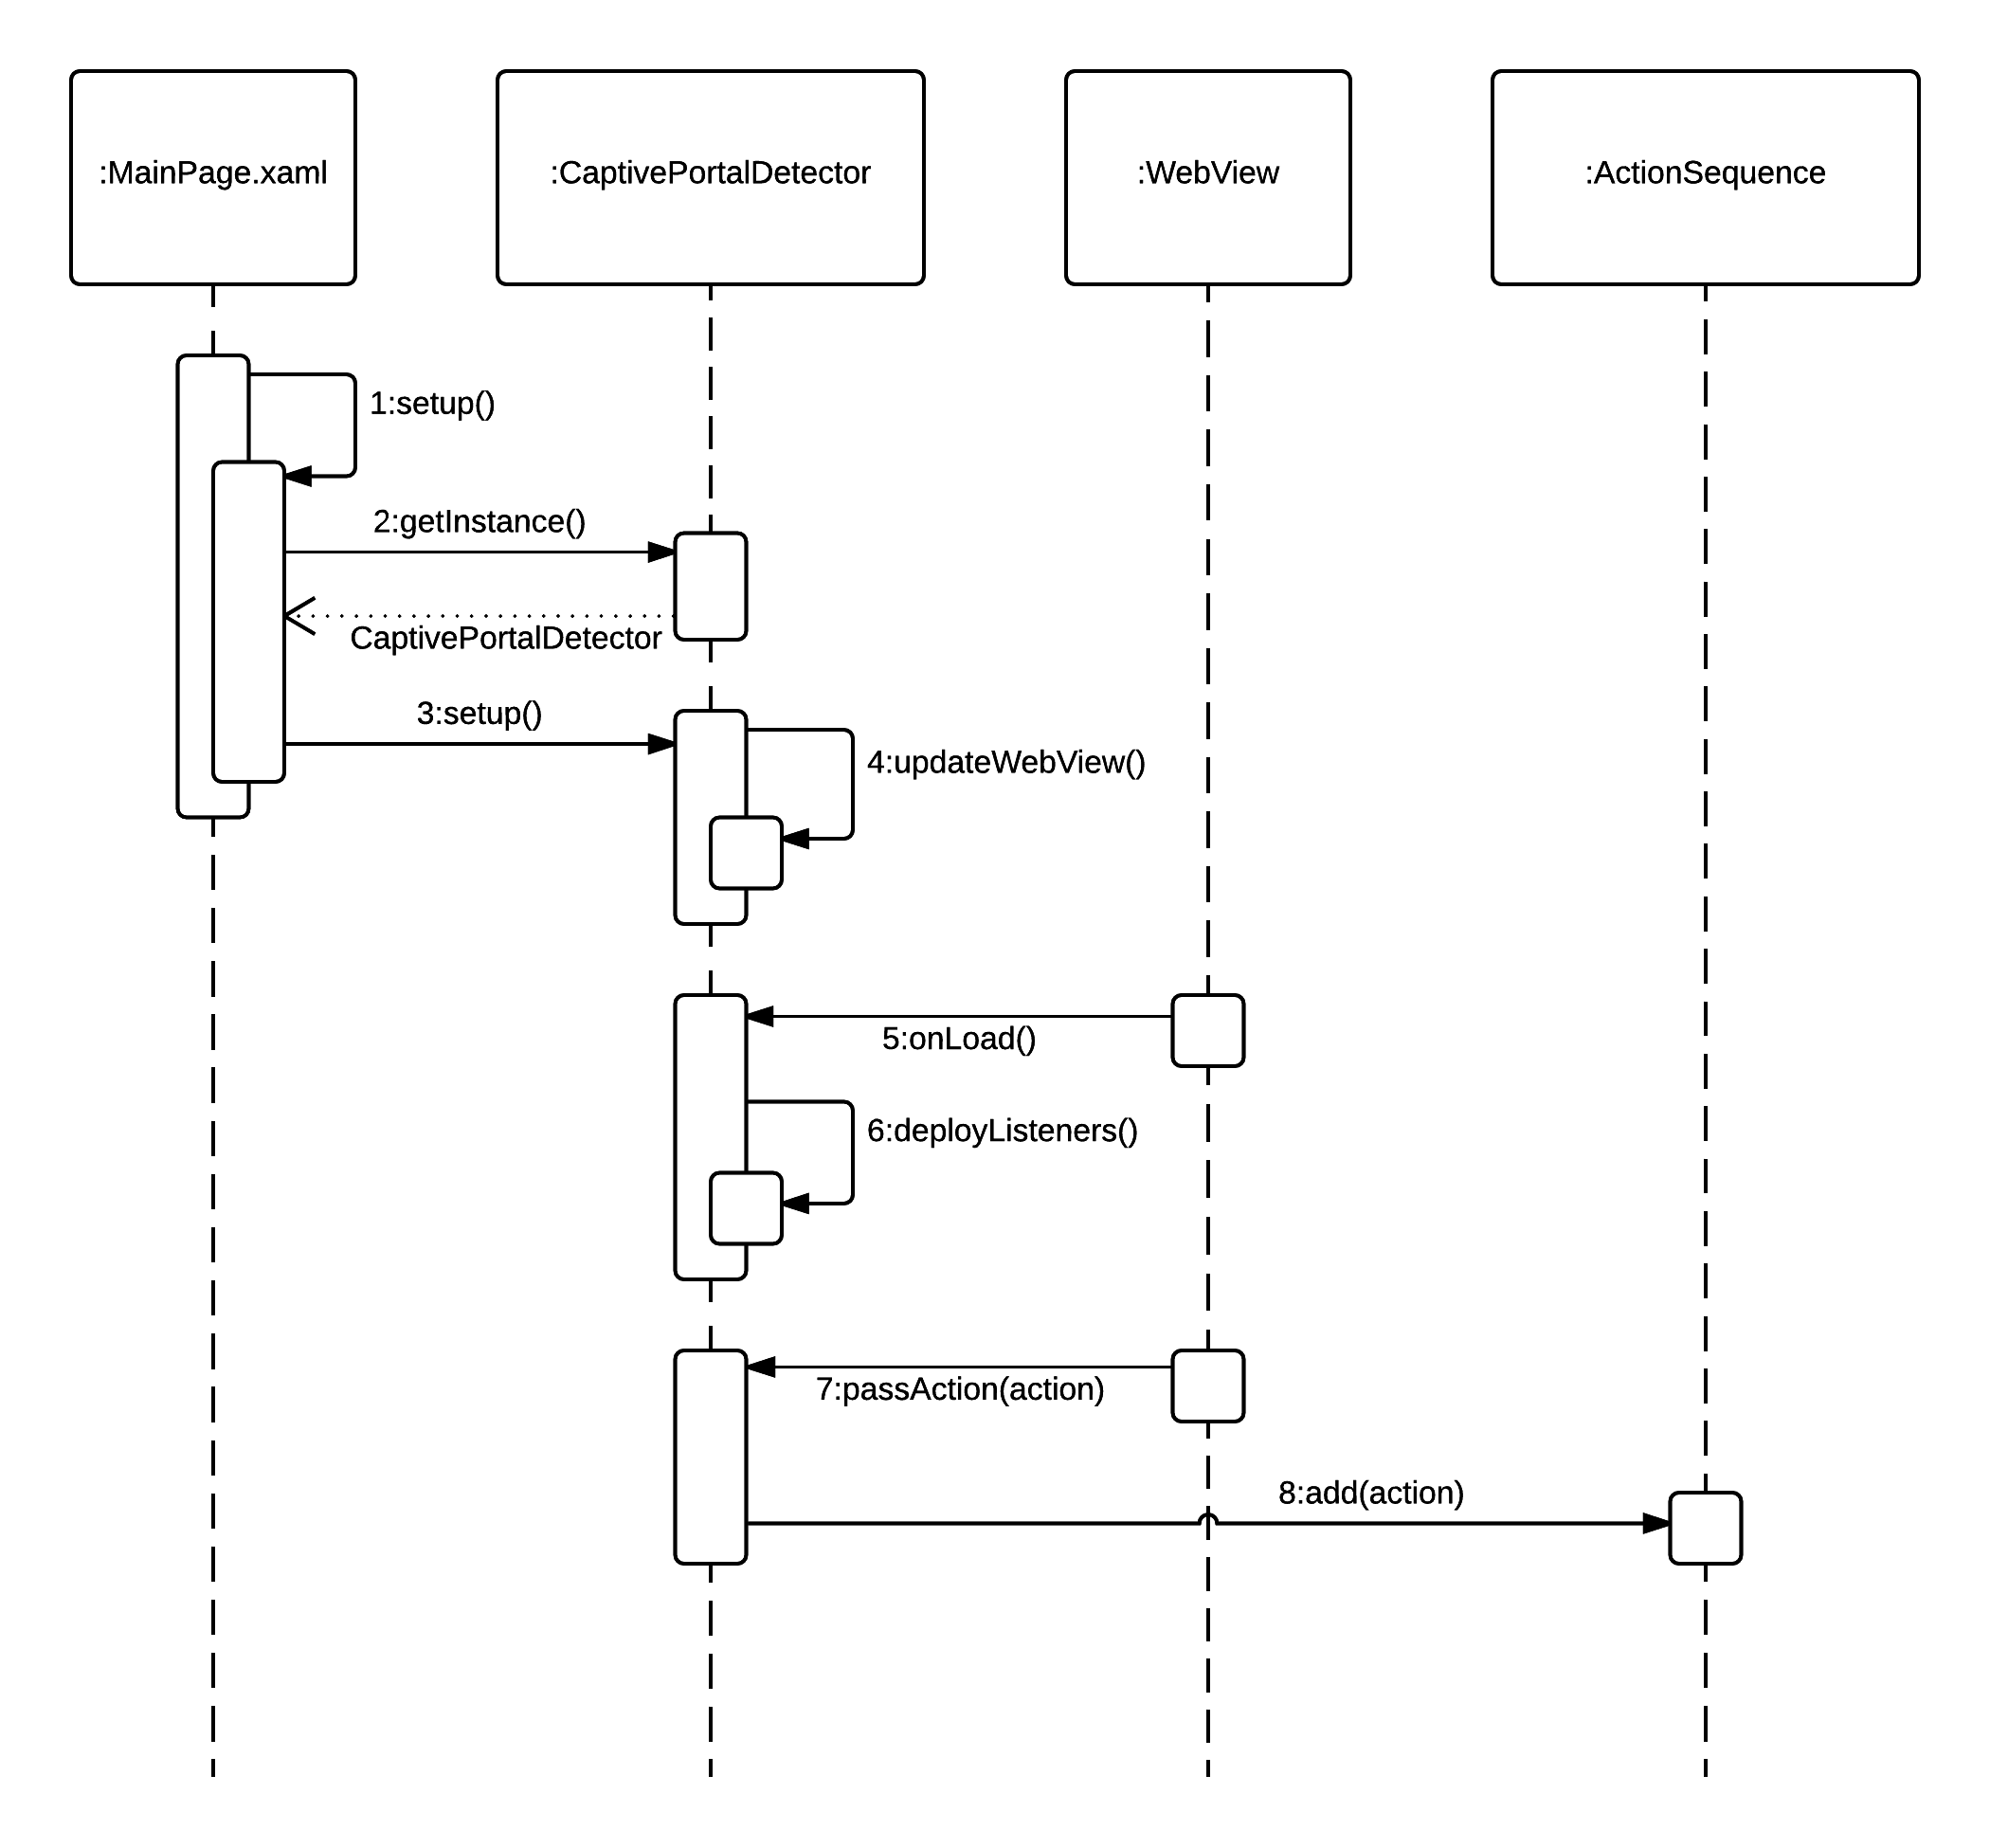
\includegraphics[scale=0.8]{Gambar/SequenceDiagramLoginInformationSaving.png}
    \caption[Diagram Interaksi Penyimpanan Informasi Login.]{Diagram Interaksi Penyimpanan Informasi Login.} 
    \label{fig:LoginInformationSavingSequenceDiagram}
\end{figure}

Gambar \ref{fig:LoginInformationSavingSequenceDiagram} menjelaskan mengenai interaksi antar objek dalam perangkat lunak untuk menyimpan informasi login. Interaksi yang terjadi adalah sebagai berikut:

\begin{enumerate}
    \item{MainPage.xaml melakukan setup().}
    \item{MainPage.xaml memanggil metode getInstance() pada kelas CaptivePortalDetector untuk mendapatkan \textit{instance} CaptivePortalDetector. MainPage.xaml mendapatkan \textit{instance} CaptivePortalDetector.}
    \item{MainPage.xaml memanggil metode setup() pada objek CaptivePortalDetector.}
    \item{CaptivePortalDetector melakukan updateWebView() untuk mengarahkan WebView ke URI yang digunakan untuk melakukan deteksi koneksi internet.}
    \item{WebView memanggil metode onLoad() pada objek CaptivePortalDetector saat halaman selesai dimuat.}
    \item{Jika halaman tidak berisi teks "connected" (tanpa tanda petik), CaptivePortalDetector melakukan deployListeners() untuk menangkap semua \textit{event} yang mungkin dilakukan oleh pengguna pada halaman tersebut.}
    \item{Metode passAction() dipanggil pada objek CaptivePortalDetector saat pengguna melakukan klik atau input teks untuk mengirimkan aksi yang baru saja dilakukan oleh pengguna.}
    \item{CaptivePortalDetector memanggil metode add() pada objek ActionSequence untuk menyimpan aksi tersebut.}
\end{enumerate}



\section{Perancangan Antarmuka}
\label{sec:perancangan_antarmuka}

Pengguna memerlukan antarmuka untuk berinteraksi dengan perangkat lunak. Antarmuka yang diperlukan adalah:

\begin{itemize}
    \item{Antarmuka notifikasi yang muncul setiap kali terhubung dengan WiFi yang menggunakan \textit{captive portal}.}
    \item{Antarmuka untuk menampilkan halaman web.}
    \item{Antarmuka untuk menampilkan pesan-pesan seperti pesan "Connected." atau "Check your network connection.".}
\end{itemize}

\subsection{Antarmuka Notifikasi}
\label{subsec:antarmuka_notifikasi}

\begin{figure}[!htb]
    \centering
    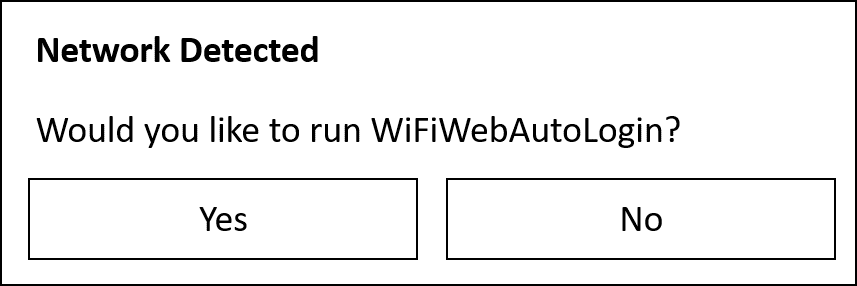
\includegraphics[scale=0.5]{Gambar/UI_Notification.png}
    \caption[Rancangan Antarmuka Notifikasi.]{Rancangan Antarmuka Notifikasi.}
    \label{fig:RancanganAntarmukaNotifikasi}
\end{figure}

Gambar \ref{fig:RancanganAntarmukaNotifikasi} menampilkan desain antarmuka notifikasi. Desain antarmuka notifikasi menggunakan desain notifikasi standar windows dengan dua tombol, "Yes" dan "No". Jika tombol "Yes" ditekan, maka notifikasi akan hilang dan aplikasi akan dijalankan. Jika tombol "No" ditekan, maka notifikasi akan hilang. Antarmuka notifikasi adalah antarmuka yang pertama kali akan muncul dalam siklus aplikasi karena kelas NetChangeDetectorBackgroundTask didaftarkan pada sistem untuk mendeteksi perubahan jaringan.

\subsection{Antarmuka Aplikasi}
\label{subsec:antarmuka_aplikasi}

Antarmuka ini digunakan untuk menampilkan halaman web dan menampilkan pesan dapat disatukan menjadi antarmuka aplikasi yang halaman kontennya dapat diubah menjadi WebView saat berada dalam mode web browser, dan menjadi Label saat berada dalam mode message box.

\subsubsection{Antarmuka Message Box}
\label{subsec:antarmuka_message_box}

\begin{figure}[!htb]
    \centering
    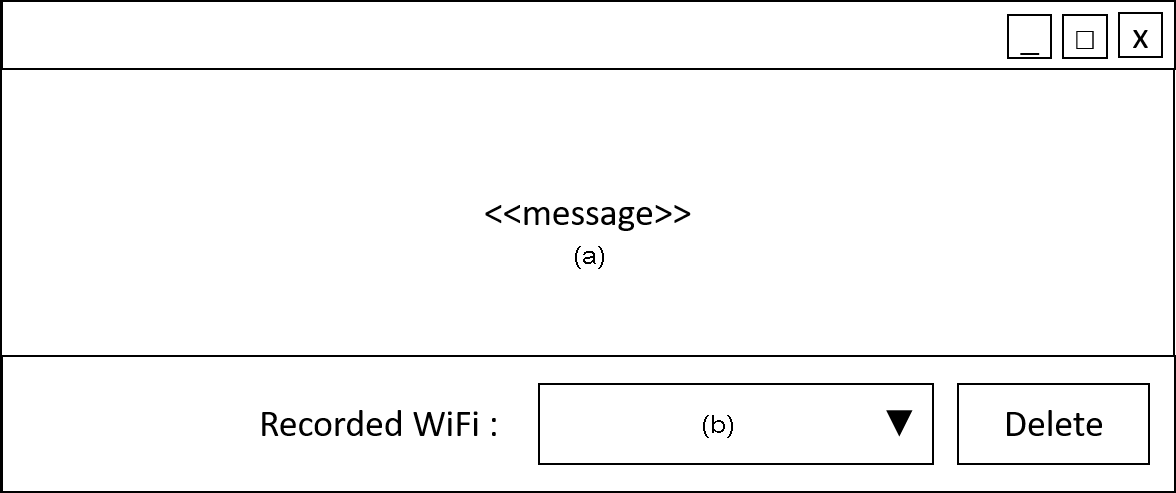
\includegraphics[scale=0.5]{Gambar/UI_MessageBox.png}
    \caption[Rancangan Antarmuka Message Box.]{Rancangan Antarmuka Message Box.}
    \label{fig:RancanganAntarmukaMessageBox}
\end{figure}

Gambar \ref{fig:RancanganAntarmukaMessageBox} menampilkan desain antarmuka message box. Selain label (a) untuk menaruh pesan, antarmuka ini juga memiliki komponen (b) untuk dapat menghapus WiFi yang sudah terekam. Dengan menghapus WiFi yang terdapat pada komponen ini, pengguna dapat merekam ulang informasi login pada WiFi tersebut.

\subsubsection{Antarmuka Web Browser}
\label{subsec:antarmuka_web_browser}

\begin{figure}[!htb]
    \centering
    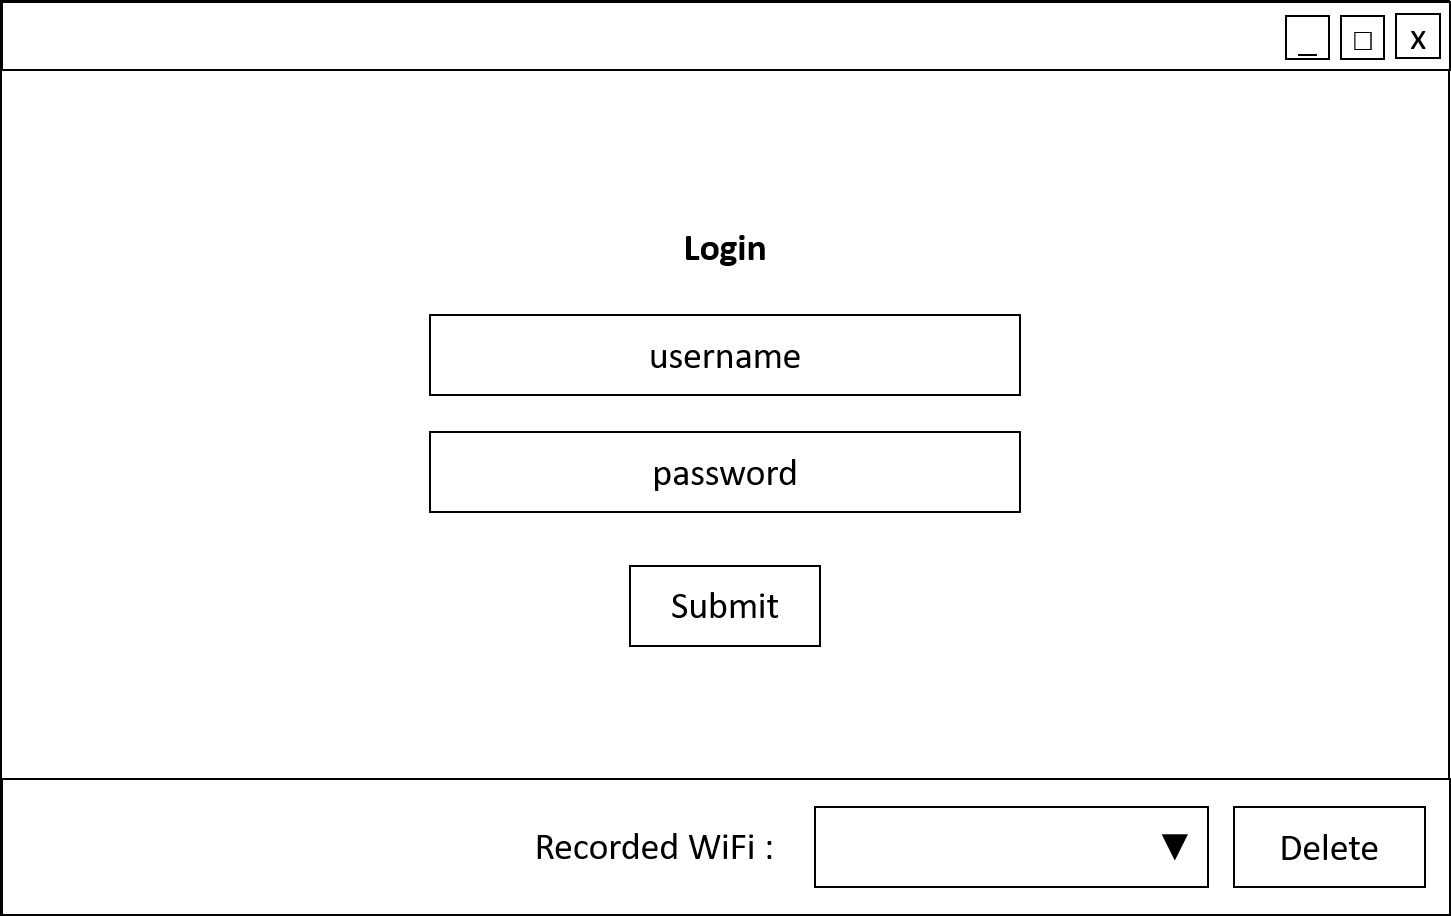
\includegraphics[scale=0.5]{Gambar/UI_WebBrowser.png}
    \caption[Rancangan Antarmuka Web Browser.]{Rancangan Antarmuka Web Browser.}
    \label{fig:RancanganAntarmukaWebBrowser}
\end{figure}

Gambar \ref{fig:RancanganAntarmukaWebBrowser} menampilkan desain antarmuka web browser. Komponen (a) digunakan untuk menampilkan halaman web yang berkaitan dengan login \textit{captive portal}. Aksi pengguna akan direkam secara otomatis pada komponen ini. Selain itu, pada antarmuka ini terdapat komponen yang sama dengan antarmuka message box, yaitu komponen (b) untuk menghapus SSID WiFi yang sudah terekam.}{}
\ifdefstring{\vbabe}{1}{\chapter{Implementasi dan Pengujian}
\label{chap:implementasi_pengujian}



\section{Masalah Implementasi dan Solusinya}
\label{sec:masalah_implementasi}

Terdapat beberapa masalah implementasi yang membuat rancangan perangkat lunak tidak dapat sepenuhnya didasarkan pada hasil analisis, di antaranya:

\begin{itemize}
    \item{Fungsi window.external.notify tidak berperilaku sebagaimana yang diperkirakan. Metode yang digunakan untuk mendapatkan hasil yang sama dengan fungsi yang diberikan oleh window.external.notify adalah dengan menggunakan kelas bertipe RuntimeComponent yang diizinkan untuk dapat diakses oleh javascript pada WebView. Kelas ini adalah ScriptNotifyHandler pada gambar \ref{fig:DetailedClassDiagram}.}
    \item{Fungsi window.open dan fungsi open tidak dapat dijalankan secara otomatis sehingga popup tidak muncul. Metode yang digunakan untuk mendapatkan hasil yang sama dari yang direncanakan sebelumnya adalah dengan melakukan \textit{override} fungsi window.open dan fungsi open dan mengubungkannya dengan kelas ScriptNotifyHandler.}
\end{itemize}

Perancangan yang tertulis pada bab 4 sudah merupakan hasil revisi dari analisis masalah implementasi ini.



\section{Rencana Pengujian}
\label{sec:rencana_pengujian}

Pengujian dalam penelitian ini dibagi menjadi dua, yaitu pengujian fungsional dan pengujian eksperimental. Pengujian fungsional dilakukan menggunakan teknik \textit{black box}. Pengujian fungsional dilakukan untuk memastikan fungsi-fungsi utama dalam perangkat lunak sudah berjalan dengan baik. Fungsi-fungsi yang akan diuji mencakupi:

\begin{itemize}
    \item{Deteksi perubahan jaringan.}
    \item{Deteksi \textit{captive portal}.}
    \item{Login otomatis.}
\end{itemize}

Setiap fungsi yang diuji diberikan kasus pengujian positif dan negatif. Sementara itu, pengujian eksperimental dilakukan untuk memeriksa apakah perangkat lunak dapat berjalan pada beragam \textit{captive portal}. Pengujian eksperimental dilakukan pada \textit{captive portal} pada jaringan WiFi dengan SSID:

\begin{itemize}
    \item{\textit{C149} pada kost di jalan Ciumbuleuit nomor 149, Bandung.}
    \item{\textit{UNPAR9} pada gedung 10 Universitas Katolik Parahyangan, Bandung.}
    \item{\textit{starbucks@wifi.id} pada Starbucks Cihampelas Walk, Bandung.}
\end{itemize}



\section{Hasil Pengujian Fungsional}
\label{sec:hasil_fungsional}

Pengujian fungsional untuk fungsi deteksi perubahan jaringan memberikan hasil sebagai berikut:

\begin{itemize}
    \item{
        \textbf{Pengujian deteksi perubahan jaringan}
        
        \begin{itemize}
            \item{
                \textbf{Pengujian positif}\\
                \textbf{Kasus}: Menghubungkan komputer dengan WiFi yang terhubung dengan \textit{captive portal}.\\
                \textbf{Hasil}: Muncul notifikasi "Network Detected" dengan pesan "Would you like to run WiFiWebAutoLogin?".
            }
            \item{
                \textbf{Pengujian negatif}\\
                \textbf{Kasus}: Menghubungkan komputer dengan WiFi yang tidak terhubung dengan \textit{captive portal}.\\
                \textbf{Hasil}: Tidak muncul notifikasi apapun.
            }
        \end{itemize}
    }
    \item{
        \textbf{Pengujian deteksi \textit{captive portal}}
        
        \begin{itemize}
            \item{
                \textbf{Pengujian positif}\\
                \textbf{Kasus}: Menghubungkan komputer dengan WiFi yang terhubung dengan \textit{captive portal} dan menekan tombol "Yes" pada notifikasi.\\
                \textbf{Hasil}: Muncul halaman login \textit{captive portal}.
            }
            \item{
                \textbf{Pengujian negatif}\\
                \textbf{Kasus}: Menghubungkan komputer dengan WiFi yang tidak terhubung dengan \textit{captive portal} maupun internet dan menekan tombol "Yes" pada notifikasi\\
                \textbf{Hasil}: Muncul pesan "Operation timeout. Check your network connection.".
            }
        \end{itemize}
    }
    \item{
        \textbf{Pengujian login otomatis}
        
        \begin{itemize}
            \item{
                \textbf{Pengujian positif}\\
                \textbf{Kasus}: Menghubungkan komputer dengan WiFi yang terhubung dengan \textit{captive portal} yang sudah pernah dijalankan login secara manual.\\
                \textbf{Hasil}: Muncul pesan "Connected.".
            }
            \item{
                \textbf{Pengujian negatif}\\
                \textbf{Kasus}: Menghubungkan komputer dengan WiFi yang terhubung dengan \textit{captive portal} yang belum pernah dijalankan login secara manual.\\
                \textbf{Hasil}: Muncul halaman login \textit{captive portal}.
            }
        \end{itemize}
    }
\end{itemize}}{}
\ifdefstring{\vbabf}{1}{\chapter{Kesimpulan dan Saran}
\label{chap:kesimpulan_dan_saran}

Bab ini memaparkan kesimpulan beserta dengan saran akan hal-hal yang dapat dilakukan untuk mengembangkan penelitian ini.



\section{Kesimpulan}
\label{sec:kesimpulan}

Beberapa hal yang dapat disimpulkan dari penelitian ini antara lain:

\begin{itemize}
    \item{Implementasi perangkat lunak untuk melakukan login otomatis pada \textit{captive portal} berhasil dilakukan walaupun memiliki keterbatasan tidak dapat melakukan login otomatis jika \textit{captive portal} menggunakan pop-up untuk mengakses halaman tujuan.}
    \item{\textit{Username} dan \textit{password} sudah disimpan secara aman dalam file yang dienkripsi menggunakan kunci yang diciptakan secara random per aplikasi.}
    \item{SSID, uri, dan konten \textit{tag} head adalah informasi yang dibutuhkan untuk membedakan antar halaman pada setiap \textit{captive portal}.}
\end{itemize}



\section{Saran}
\label{sec:saran}

Saran yang dapat dilakukan untuk mengembangkan penelitian ini adalah gunakan \textit{platform} lain selain UWP, seperti Windows Form, Java, Android, atau iOS. Hal ini dapat dilakukan untuk menghindari keterbatasan WebView pada UWP dalam menangani pop-up.}{}
\ifdefstring{\vbabg}{1}{\include{Bab/bab7}}{}
\ifdefstring{\vbabh}{1}{\include{Bab/bab8}}{}
\ifdefstring{\vbabi}{1}{\include{Bab/bab9}}{}

\bibliographystyle{ieeetr}
\bibliography{pustaka}

\appendix
\apptoc

\tampillmp{\vlmp}
\ifdefstring{\vlmpa}{1}{\chapter{Kode Sumber}
\label{lampiran:A}



\section{Namespace: WiFiWebAutoLogin}
\label{namespace:WiFiWebAutoLogin}

\kodesumber{xml}{WiFiWebAutoLogin/Package.appxmanifest}
\kodesumber{xml}{WiFiWebAutoLogin/App.xaml}
\kodesumber{csharp}{WiFiWebAutoLogin/App.xaml.cs}
\kodesumber{xml}{WiFiWebAutoLogin/MainPage.xaml}
\kodesumber{csharp}{WiFiWebAutoLogin/MainPage.xaml.cs}
\kodesumber{javascript}{WiFiWebAutoLogin/JavaScript/DeployListeners.js}



\section{Namespace: WiFiWebAutoLogin.Classes}
\label{namespace:WiFiWebAutoLogin.Classes}

\kodesumber{csharp}{WiFiWebAutoLogin.Classes/ActionSequence.cs}
\kodesumber{csharp}{WiFiWebAutoLogin.Classes/CaptivePortalDetector.cs}
\kodesumber{csharp}{WiFiWebAutoLogin.Classes/Conf.cs}
\kodesumber{csharp}{WiFiWebAutoLogin.Classes/LoginInformation.cs}
\kodesumber{csharp}{WiFiWebAutoLogin.Classes/Storage.cs}



\section{Namespace: WiFiWebAutoLogin.RuntimeComponents}
\label{namespace:WiFiWebAutoLogin.RuntimeComponents}

\kodesumber{csharp}{WiFiWebAutoLogin.RuntimeComponents/NetChangeDetectorBackgroundTask.cs}
\kodesumber{csharp}{WiFiWebAutoLogin.RuntimeComponents/ScriptNotifyHandler.cs}}{}
\ifdefstring{\vlmpb}{1}{%\chapter{The Source Code}
%\label{app:B}
%
%%selalu gunakan single spacing untuk source code !!!!!
%\singlespacing 
%% language: bahasa dari kode program
%% terdapat beberapa pilihan : Java, C, C++, PHP, Matlab, R, dll
%%
%% basicstyle : ukuran font untuk kode program
%% terdapat beberapa pilihan : tiny, scriptsize, footnotesize, dll
%%
%% caption : nama yang akan ditampilkan di dokumen akhir, lihat contoh
%\begin{lstlisting}[language=Java,basicstyle=\tiny,caption=MyFurSet.java]
%
%import java.util.ArrayList;
%import java.util.Collections;
%import java.util.HashSet;
%
%/**
 %*
 %* @author Lionov
 %*/
%
%//class for set of vertices close to furthest edge
%public class MyFurSet {
    %protected int id;                                  //id of the set
    %protected MyEdge FurthestEdge;                     //the furthest edge
    %protected HashSet<MyVertex> set;                   //set of vertices close to furthest edge
    %protected ArrayList<ArrayList<Integer>> ordered;   //list of all vertices in the set for each trajectory
    %protected ArrayList<Integer> closeID;              //store the ID of all vertices
    %protected ArrayList<Double> closeDist;             //store the distance of all vertices
    %protected int totaltrj;                            //total trajectories in the set
%
    %/**
     %* Constructor
     %* @param id : id of the set
     %* @param totaltrj : total number of trajectories in the set
     %* @param FurthestEdge : the furthest edge
     %*/
    %public MyFurSet(int id,int totaltrj,MyEdge FurthestEdge) {
        %this.id = id;
        %this.totaltrj = totaltrj;
        %this.FurthestEdge = FurthestEdge;
        %set = new HashSet<MyVertex>();
        %ordered = new ArrayList<ArrayList<Integer>>();
        %for (int i=0;i<totaltrj;i++) ordered.add(new ArrayList<Integer>());
        %closeID = new ArrayList<Integer>(totaltrj);
        %closeDist = new ArrayList<Double>(totaltrj);
        %for (int i = 0;i <totaltrj;i++) {
            %closeID.add(-1);
            %closeDist.add(Double.MAX_VALUE);
        %}
    %}
%
    %/**
     %* set a vertex into the set
     %* @param v : vertex to be added to the set
     %*/
    %public void add(MyVertex v) {
        %set.add(v);
    %}
%
    %/**
     %* check whether vertex v is a member of the set
     %* @param v : vertex to be checked
     %* @return true if v is a member of the set, false otherwise
     %*/
    %public boolean contains(MyVertex v) {
        %return this.set.contains(v);
    %}
%}
%\end{lstlisting}}{}
\ifdefstring{\vlmpc}{1}{\include{Lampiran/lampC}}{}
\ifdefstring{\vlmpd}{1}{\include{Lampiran/lampD}}{}
\ifdefstring{\vlmpe}{1}{\include{Lampiran/lampE}}{}
\ifdefstring{\vlmpf}{1}{\include{Lampiran/lampF}}{}
\ifdefstring{\vlmpg}{1}{\include{Lampiran/lampG}}{}
\ifdefstring{\vlmph}{1}{\include{Lampiran/lampH}}{}
\ifdefstring{\vlmpi}{1}{\include{Lampiran/lampI}}{}

\end{document}

%=============================================================================
% Perubahan pada versi 8 (31-05-2015): 
%	- penambahan default data untuk beberapa keterangan dan digunakan sebagai 
%	  template dengan tanda << & >> . Data yang diubah defaultnya adalah: nama skripsi
%	  nama prodi, beserta bahasa inggrisnya.
%   - Keywords dan kata kunci di abstrak ditambahkan noindent + perbaikan lainnya
%   - Perbaikan untuk halaman tidak kosong tanpa nomor halaman romawi
% Perubahan pada versi 7 (27-05-2014)
%	- penambahan perintah \raggedbottom untuk menghilangkan area kosong akibat 
%	  penempatan gambar yang tidak sempurna
% Perubahan pada versi 6 (10-11-2013)
%	- perbaikan pada abstract dengan paragraf lebih dari satu: perbaikan vertical spacing
%	- perbaikan pada tampilan bab dan lampiran: tidak perlu menuliskan apapun untuk 
%	  menampilkan semuanya (di data.tex) atau -1 jika tidak ada lampiran
%	- halaman bernomor genap untuk halaman romawi sudah dimunculkan
%	- Kurikulum 2013 : perubahan nama buku skripsi 
% Perubahan pada versi 5 (21-10-2012)
%	- halaman terakhir setiap bab tidak ada headernya jika kosong
% Perubahan pada versi 4 (06-08-2012)
% 	- penggabungan main.tex, depan.tex dan setup.tex menjadi main.tex
% 	- menambahkan keterangan di lampiran untuk kode program 
% 	- ukuran font dapat diubah langsung di tiap lampiran
% Perubahan pada versi 3 (09-07-2012): 
%	- Tidak ada perubahan di file ini
% Perubahan pada versi 2 (08-07-2012):
% 	- "Daftar Referensi" tidak perlu diubah secara manual (tidak perlu mengubah file bahasai.ldf)
% 	- Bahasa Indonesia dari abstract adalah abstrak (secara otomatis), bukan ringkasan
% 	- Spasi pada buku dokumen final adalah onehalfspacing
% Versi 1 (08-11-2011)
%=============================================================================
%=============================================================================
% depan.tex v2 (09-07-2012)
% Perubahan pada versi 2:
% - Menambahkan halaman depan dalam bahasa inggris
% Versi 1 (08-11-2011)
%=============================================================================
% setup.tex v2 (08-07-2012)
% Perubahan pada versi 2:
% - Menambahkan perintah untuk judulINA dan judulENG
% - Menghapus \usepackage{microtype}, yang pada beberapa kasus menjadi masalah
% Versi 1 (08-11-2011)
%=============================================================================